% uWaterloo Thesis Template for LaTeX 
% Last Updated May 24, 2011 by Stephen Carr, IST Client Services
% FOR ASSISTANCE, please send mail to rt-IST-CSmathsci@ist.uwaterloo.ca

% Effective October 2006, the University of Waterloo 
% requires electronic thesis submission. See the uWaterloo thesis regulations at
% http://www.grad.uwaterloo.ca/Thesis_Regs/thesistofc.asp.

% DON'T FORGET TO ADD YOUR OWN NAME AND TITLE in the "hyperref" package
% configuration below. THIS INFORMATION GETS EMBEDDED IN THE PDF FINAL PDF DOCUMENT.
% You can view the information if you view Properties of the PDF document.

% Many faculties/departments also require one or more printed
% copies. This template attempts to satisfy both types of output. 
% It is based on the standard "book" document class which provides all necessary 
% sectioning structures and allows multi-part theses.

% DISCLAIMER
% To the best of our knowledge, this template satisfies the current uWaterloo requirements.
% However, it is your responsibility to assure that you have met all 
% requirements of the University and your particular department.
% Many thanks to the feedback from many graduates that assisted the development of this template.

% -----------------------------------------------------------------------

% By default, output is produced that is geared toward generating a PDF 
% version optimized for viewing on an electronic display, including 
% hyperlinks within the PDF.
 
% E.g. to process a thesis called "mythesis.tex" based on this template, run:

% pdflatex mythesis	-- first pass of the pdflatex processor
% bibtex mythesis	-- generates bibliography from .bib data file(s) 
% pdflatex mythesis	-- fixes cross-references, bibliographic references, etc
% pdflatex mythesis	-- fixes cross-references, bibliographic references, etc

% If you use the recommended LaTeX editor, Texmaker, you would open the mythesis.tex
% file, then click the pdflatex button. Then run BibTeX (under the Tools menu).
% Then click the pdflatex button two more times. If you have an index as well,
% you'll need to run MakeIndex from the Tools menu as well, before running pdflatex
% the last two times.

% N.B. The "pdftex" program allows graphics in the following formats to be
% included with the "\includegraphics" command: PNG, PDF, JPEG, TIFF
% Tip 1: Generate your figures and photos in the size you want them to appear
% in your thesis, rather than scaling them with \includegraphics options.
% Tip 2: Any drawings you do should be in scalable vector graphic formats:
% SVG, PNG, WMF, EPS and then converted to PNG or PDF, so they are scalable in
% the final PDF as well.
% Tip 3: Photographs should be cropped and compressed so as not to be too large.

% To create a PDF output that is optimized for double-sided printing: 
%
% 1) comment-out the \documentclass statement in the preamble below, and
% un-comment the second \documentclass line.
%
% 2) change the value assigned below to the boolean variable
% "PrintVersion" from "false" to "true".

% --------------------- Start of Document Preamble -----------------------

% Specify the document class, default style attributes, and page dimensions
% For hyperlinked PDF, suitable for viewing on a computer, use this:
\documentclass[letterpaper,12pt,titlepage,oneside,final]{book}
 
% For PDF, suitable for double-sided printing, change the PrintVersion variable below
% to "true" and use this \documentclass line instead of the one above:
%\documentclass[letterpaper,12pt,titlepage,openright,twoside,final]{book}

% Some LaTeX commands I define for my own nomenclature.
% If you have to, it's better to change nomenclature once here than in a 
% million places throughout your thesis!
\newcommand{\package}[1]{\textbf{#1}} % package names in bold text
\newcommand{\cmmd}[1]{\textbackslash\texttt{#1}} % command name in tt font 
\newcommand{\href}[1]{#1} % does nothing, but defines the command so the
    % print-optimized version will ignore \href tags (redefined by hyperref pkg).
%\newcommand{\texorpdfstring}[2]{#1} % does nothing, but defines the command
% Anything defined here may be redefined by packages added below...

% This package allows if-then-else control structures.
\usepackage{ifthen}
\newboolean{PrintVersion}
\setboolean{PrintVersion}{false} 
% CHANGE THIS VALUE TO "true" as necessary, to improve printed results for hard copies
% by overriding some options of the hyperref package below.

%\usepackage{nomencl} % For a nomenclature (optional; available from ctan.org)
\usepackage{amsmath,amssymb,amstext} % Lots of math symbols and environments
\usepackage[pdftex]{graphicx} % For including graphics N.B. pdftex graphics driver 

%MY MACROS
%————————————————
\usepackage{algorithm}
\usepackage{algpseudocode}
\usepackage{theorem}
\usepackage{tikz}
\usepackage{tkz-berge}

%Macros
\newcommand{\A}{\mathbb{A}} \newcommand{\C}{\mathbb{C}}
\newcommand{\D}{\mathbb{D}} \newcommand{\F}{\mathbb{F}}
\newcommand{\N}{\mathbb{N}} \newcommand{\R}{\mathbb{R}}
\newcommand{\T}{\mathbb{T}} \newcommand{\Z}{\mathbb{Z}}
\newcommand{\Q}{\mathbb{Q}}
 
 
\newcommand{\cA}{\mathcal{A}} \newcommand{\cB}{\mathcal{B}}
\newcommand{\cC}{\mathcal{C}} \newcommand{\cD}{\mathcal{D}}
\newcommand{\cE}{\mathcal{E}} \newcommand{\cF}{\mathcal{F}}
\newcommand{\cG}{\mathcal{G}} \newcommand{\cH}{\mathcal{H}}
\newcommand{\cI}{\mathcal{I}} \newcommand{\cJ}{\mathcal{J}}
\newcommand{\cK}{\mathcal{K}} \newcommand{\cL}{\mathcal{L}}
\newcommand{\cM}{\mathcal{M}} \newcommand{\cN}{\mathcal{N}}
\newcommand{\cO}{\mathcal{O}} \newcommand{\cP}{\mathcal{P}}
\newcommand{\cQ}{\mathcal{Q}} \newcommand{\cR}{\mathcal{R}}
\newcommand{\cS}{\mathcal{S}} \newcommand{\cT}{\mathcal{T}}
\newcommand{\cU}{\mathcal{U}} \newcommand{\cV}{\mathcal{V}}
\newcommand{\cW}{\mathcal{W}} \newcommand{\cX}{\mathcal{X}}
\newcommand{\cY}{\mathcal{Y}} \newcommand{\cZ}{\mathcal{Z}}

\newcommand\numberthis{\addtocounter{equation}{1}\tag{\theequation}}


\newenvironment{proof}{{\bf Proof:  }}{\hfill\rule{2mm}{2mm}}
\newenvironment{proofof}[1]{{\bf Proof of #1:  }}{\hfill\rule{2mm}{2mm}}
\newenvironment{proofofnobox}[1]{{\bf#1:  }}{}\newenvironment{example}{{\bf Example:  }}{\hfill\rule{2mm}{2mm}}

%\renewcommand{\thesection}{\lecnum.\arabic{section}}
%\renewcommand{\theequation}{\thesection.\arabic{equation}}
%\renewcommand{\thefigure}{\thesection.\arabic{figure}}

\newtheorem{fact}{Fact}[section]
\newtheorem{lemma}[fact]{Lemma}
\newtheorem{theorem}[fact]{Theorem}
\newtheorem{definition}[fact]{Definition}
\newtheorem{corollary}[fact]{Corollary}
\newtheorem{proposition}[fact]{Proposition}
\newtheorem{claim}[fact]{Claim}
\newtheorem{exercise}[fact]{Exercise}
\newtheorem{note}[fact]{Note}
\newtheorem{conjecture}[fact]{Conjecture}

\newcommand{\size}[1]{\ensuremath{\left|#1\right|}}
\newcommand{\ceil}[1]{\ensuremath{\left\lceil#1\right\rceil}}
\newcommand{\floor}[1]{\ensuremath{\left\lfloor#1\right\rfloor}}

%END MACROS
%—————————————————————————————————

% Hyperlinks make it very easy to navigate an electronic document.
% In addition, this is where you should specify the thesis title
% and author as they appear in the properties of the PDF document.
% Use the "hyperref" package 
% N.B. HYPERREF MUST BE THE LAST PACKAGE LOADED; ADD ADDITIONAL PKGS ABOVE
\usepackage[pdftex,letterpaper=true,pagebackref=false]{hyperref} % with basic options
		% N.B. pagebackref=true provides links back from the References to the body text. This can cause trouble for printing.
\hypersetup{
    plainpages=false,       % needed if Roman numbers in frontpages
    pdfpagelabels=true,     % adds page number as label in Acrobat's page count
    bookmarks=true,         % show bookmarks bar?
    unicode=false,          % non-Latin characters in Acrobat’s bookmarks
    pdftoolbar=true,        % show Acrobat’s toolbar?
    pdfmenubar=true,        % show Acrobat’s menu?
    pdffitwindow=false,     % window fit to page when opened
    pdfstartview={FitH},    % fits the width of the page to the window
    pdftitle={uWaterloo\ LaTeX\ Thesis\ Template},    % title: CHANGE THIS TEXT!
%    pdfauthor={Author},    % author: CHANGE THIS TEXT! and uncomment this line
%    pdfsubject={Subject},  % subject: CHANGE THIS TEXT! and uncomment this line
%    pdfkeywords={keyword1} {key2} {key3}, % list of keywords, and uncomment this line if desired
    pdfnewwindow=true,      % links in new window
    colorlinks=true,        % false: boxed links; true: colored links
    linkcolor=blue,         % color of internal links
    citecolor=green,        % color of links to bibliography
    filecolor=magenta,      % color of file links
    urlcolor=cyan           % color of external links
}
\ifthenelse{\boolean{PrintVersion}}{   % for improved print quality, change some hyperref options
\hypersetup{	% override some previously defined hyperref options
%    colorlinks,%
    citecolor=black,%
    filecolor=black,%
    linkcolor=black,%
    urlcolor=black}
}{} % end of ifthenelse (no else)

% Setting up the page margins...
% uWaterloo thesis requirements specify a minimum of 1 inch (72pt) margin at the
% top, bottom, and outside page edges and a 1.125 in. (81pt) gutter
% margin (on binding side). While this is not an issue for electronic
% viewing, a PDF may be printed, and so we have the same page layout for
% both printed and electronic versions, we leave the gutter margin in.
% Set margins to minimum permitted by uWaterloo thesis regulations:
\setlength{\marginparwidth}{0pt} % width of margin notes
% N.B. If margin notes are used, you must adjust \textwidth, \marginparwidth
% and \marginparsep so that the space left between the margin notes and page
% edge is less than 15 mm (0.6 in.)
\setlength{\marginparsep}{0pt} % width of space between body text and margin notes
\setlength{\evensidemargin}{0.125in} % Adds 1/8 in. to binding side of all 
% even-numbered pages when the "twoside" printing option is selected
\setlength{\oddsidemargin}{0.125in} % Adds 1/8 in. to the left of all pages
% when "oneside" printing is selected, and to the left of all odd-numbered
% pages when "twoside" printing is selected
\setlength{\textwidth}{6.375in} % assuming US letter paper (8.5 in. x 11 in.) and 
% side margins as above
\raggedbottom

% The following statement specifies the amount of space between
% paragraphs. Other reasonable specifications are \bigskipamount and \smallskipamount.
\setlength{\parskip}{\medskipamount}

% The following statement controls the line spacing.  The default
% spacing corresponds to good typographic conventions and only slight
% changes (e.g., perhaps "1.2"), if any, should be made.
\renewcommand{\baselinestretch}{1} % this is the default line space setting

% By default, each chapter will start on a recto (right-hand side)
% page.  We also force each section of the front pages to start on 
% a recto page by inserting \cleardoublepage commands.
% In many cases, this will require that the verso page be
% blank and, while it should be counted, a page number should not be
% printed.  The following statements ensure a page number is not
% printed on an otherwise blank verso page.
\let\origdoublepage\cleardoublepage
\newcommand{\clearemptydoublepage}{%
  \clearpage{\pagestyle{empty}\origdoublepage}}
\let\cleardoublepage\clearemptydoublepage

%======================================================================
%   L O G I C A L    D O C U M E N T -- the content of your thesis
%======================================================================
\begin{document}

% For a large document, it is a good idea to divide your thesis
% into several files, each one containing one chapter.
% To illustrate this idea, the "front pages" (i.e., title page,
% declaration, borrowers' page, abstract, acknowledgements,
% dedication, table of contents, list of tables, list of figures,
% nomenclature) are contained within the file "uw-ethesis-frontpgs.tex" which is
% included into the document by the following statement.
%----------------------------------------------------------------------
% FRONT MATERIAL
%----------------------------------------------------------------------
% T I T L E   P A G E
% -------------------
% Last updated May 24, 2011, by Stephen Carr, IST-Client Services
% The title page is counted as page `i' but we need to suppress the
% page number.  We also don't want any headers or footers.
\pagestyle{empty}
\pagenumbering{roman}

% The contents of the title page are specified in the "titlepage"
% environment.
\begin{titlepage}
        \begin{center}
        \vspace*{1.0cm}

        \Huge
        {\bf Structure in Stable Matching Problems }

        \vspace*{1.0cm}

        \normalsize
        by \\

        \vspace*{1.0cm}

        \Large
        William Justin Toth \\

        \vspace*{3.0cm}

        \normalsize
        A thesis \\
        presented to the University of Waterloo \\ 
        in fulfillment of the \\
        thesis requirement for the degree of \\
        Master of Mathematics \\
        in \\
        Combinatorics and Optimization \\

        \vspace*{2.0cm}

        Waterloo, Ontario, Canada, 2016 \\

        \vspace*{1.0cm}

        \copyright\ William Justin Toth 2016 \\
        \end{center}
\end{titlepage}

% The rest of the front pages should contain no headers and be numbered using Roman numerals starting with `ii'
\pagestyle{plain}
\setcounter{page}{2}

\cleardoublepage % Ends the current page and causes all figures and tables that have so far appeared in the input to be printed.
% In a two-sided printing style, it also makes the next page a right-hand (odd-numbered) page, producing a blank page if necessary.
 


% D E C L A R A T I O N   P A G E
% -------------------------------
  % The following is the sample Delaration Page as provided by the GSO
  % December 13th, 2006.  It is designed for an electronic thesis.
  \noindent
I hereby declare that I am the sole author of this thesis. This is a true copy of the thesis, including any required final revisions, as accepted by my examiners.

  \bigskip
  
  \noindent
I understand that my thesis may be made electronically available to the public.

\cleardoublepage
%\newpage

% A B S T R A C T
% ---------------

\begin{center}\textbf{Abstract}\end{center}

\paragraph{}
In this thesis we provide two contributions to the study of structure in stable matching problems. First, a short new proof for the integrality of
  Rothblum's linear description of the convex hull of incidence
  vectors of stable matchings in bipartite graphs. The key feature of our proof is to show
  that extreme points of the formulation must have a $0,1$-component. 
  \paragraph{}
  Second, a computer search procedure for instances of cyclic stable matching problems with three genders as proposed by Knuth. We provide sufficient conditions for the existence of a stable matching in this context. We also investigate bijections of the problem instance vertex set to itself which preserve the set of stable matchings (up to permutation). Such bijections define ``symmetric" problem instances. We study this notion of symmetry, and use it to cut down on the number of problem instances in our search. We implemented our proposed computational procedure in Java and end with a discussion of the results running computational experiments using our code on problem instances of size $5$.
\cleardoublepage
%\newpage

% A C K N O W L E D G E M E N T S
% -------------------------------

\begin{center}\textbf{Acknowledgements}\end{center}

I would like to thank Jochen Koenemann and Kanstantsin Pashkovich. Their guidance has been invaluable.
\cleardoublepage
%\newpage

% D E D I C A T I O N
% -------------------

\begin{center}\textbf{Dedication}\end{center}

This is dedicated to my parents Bill and Cheryl, and my brother Michael, for their unwavering support in all my endeavours.
\cleardoublepage
%\newpage

% T A B L E   O F   C O N T E N T S
% ---------------------------------
\renewcommand\contentsname{Table of Contents}
\tableofcontents
\cleardoublepage
\phantomsection
%\newpage

% L I S T   O F   T A B L E S
% ---------------------------
%\addcontentsline{toc}{chapter}{List of Tables}
%\listoftables
%\cleardoublepage
%\phantomsection		% allows hyperref to link to the correct page
%\newpage

% L I S T   O F   F I G U R E S
% -----------------------------
\addcontentsline{toc}{chapter}{List of Figures}
\listoffigures
\cleardoublepage
\phantomsection		% allows hyperref to link to the correct page
%\newpage

% L I S T   O F   S Y M B O L S
% -----------------------------
% To include a Nomenclature section
% \addcontentsline{toc}{chapter}{\textbf{Nomenclature}}
% \renewcommand{\nomname}{Nomenclature}
% \printglossary
% \cleardoublepage
% \phantomsection % allows hyperref to link to the correct page
% \newpage

% Change page numbering back to Arabic numerals
\pagenumbering{arabic}

 

%----------------------------------------------------------------------
% MAIN BODY
%----------------------------------------------------------------------
% Because this is a short document, and to reduce the number of files
% needed for this template, the chapters are not separate
% documents as suggested above, but you get the idea. If they were
% separate documents, they would each start with the \chapter command, i.e, 
% do not contain \documentclass or \begin{document} and \end{document} commands.

%======================================================================
%INTRODUCTION
%======================================================================
%======================================================================
\chapter{Introduction}
%======================================================================
This chapter gives motivation, history of related work, and how our results fit into the current body of knowledge.

%----------------------------------------------------------------------
\section{Motivation and Related Work}

\paragraph{}
These days online dating applications are all the rage for eligible singles, but before these apps made finding a date as easy as a swipe of the finger, one way people met potential suitors was through their social circle. Imagine you really like playing cupid and you happen to know $n$ heterosexual male and heterosexual female friends who are all single and looking for dates. Since you're such a good friend you know each of your friends preferences over who they would like to be paired with in the opposite gender, and even who they deem unacceptable. You would like to set up your single friends together in $n$ pairs and you have a goal: you don't want your friends to mutually circumvent your dating suggestions. Say some are your friends are Adam, Bob, Amy, and Brianne. If you pair Adam and Amy together, and Bob and Brianne, but Adam and Brianne mutually prefer each other to Amy and Bob respectively then they might want to ditch their suggested dates for each other. You hope to avoid this.
\paragraph{}
In the previous dating game your single friends with their preferences form what is called by economists a two-sided matching market \cite{roth1992two}. The hope that your friends don't mutually want to ditch their dates is the condition of stability which is a highly desirable property in matching markets. A pair of friends who mutually prefer each other to their matches are called a blocking pair, and the existence of a blocking pair prevents stability. Other (perhaps more practical) examples two-sided matching markets are the matching of medical school residents with hospitals for internships, college applicants with colleges, and labour markets between employers and employees. The critical features of two-sided matching markets are the presence of two distinct groups without crossover who have interests in forming some mutual relationship with a member of the opposite group, and not only that but each member has preferences who they become involved with in the opposite group.
\paragraph{}
The abstract mathematical model of these phenomena is called a stable matching problem. In particular the model with two sides and strict preferences, referred to as Stable Marriage was first introduced by Gale and Shapley to investigate college admissions \cite{gale1962college}. In Gale and Shapley's work they prove that stable matchings always exist for stable marriage problems through giving their famous deferred acceptance algorithm to compute stable matchings. Their groundbreaking work earned them the Nobel Prize in Economics. Perhaps more significant than that they spawned a field of inquiry that brings together mathematicians, computer scientists, and economists in studying stable matching problems and their variants.
\paragraph{}
Stable matching in two-sided markets come with a lot of interesting structure. In Gale and Shapley's original paper they observed that their algorithm favoured one side of the market over the other. Deferred acceptance has one side of the market play the role of proposers, as it turns out the algorithm gives the proposers the best possible partner they could hope for in any stable matching. McVitie and Wilson \cite{mcvitie1971stable} gave an algorithm which found not just one stable matching for a market, but all of them. They also observed that in a stable matching where one side of the market are all matched with their best possible partner, like in deferred acceptance, the other side of the market are all matched with their worst possible partner. Another interesting structural result came from Gale and Sotomayor \cite{gale1985some} when they demonstrated that if someone was matched in any stable matching they were matched in all stable matchings. An immediate corollary of which is that all stable matchings of a given market have the same size. 
\paragraph{}
A major landmark in stable marriage was the work of Knuth \cite{knuthmariages}. Knuth extended the observations of McVitie and Wilson by demonstrating that when given two stable matchings, if all members of one side of the market like the first stable matching at least as well as the second then all members of the other side of the market like the second stable matching at least as well as the first. In plainer language the interests of both sides of the market are opposed. In his work Knuth also mentions that the set of stable matchings of a two-sided market form an algebraic structure called a distributive lattice. He credits Conway with the result. Blair takes this result further and demonstrates the amazing fact that any finite distributive lattice is equivalent to the set of stable matchings of some two-sided market \cite{blair1984every}.
\paragraph{}
One natural question which arises when first hearing about stable matching is: what happens when we remove sides from the market? That is, what happens when we allow all participants in the market to match with any other participant? This problem has been given the evocative name Stable Roommates problem. In Gale and Shapley's original work \cite{gale1962college} they give consider this problem and give a example which shows the existence of a problem instance where no stable matching is possible.  Abeledo and Isaak advance this further by proving that your matching market is two-sided if and only if for any reordering of the participants preferences over who they are matched with the resulting market has a stable matching \cite{abeledo1991characterization}.
\paragraph{}
In the stable roommates problem we would like an algorithm like the deferred acceptance procedure of Gale and Shapley that provides stable matchings, but since not every problem instance has a stable matching the algorithm should also be able to decide when a stable matching does not exist. In 1985, Irving provided such an algorithm \cite{irving1985efficient}. In collaboration with Gusfield \cite{irving1987efficient}, Irving showed as a consequence of his algorithm that for any stable roommates instance if a participant is matched in a stable matching they are matched in all stable matchings. As a corollary this implies that stable matchings in a given market all have the same size. Despite Irving's efficient algorithm, it is $NP$-hard to find a matching with the least number of pairs blocking the matching \cite{abraham2005almost}. For those without a complexity background, an optimization problem being $NP$-hard is considered strong evidence that no efficient algorithm exists for that problem. By efficient we mean that worst case running is bounded above by a polynomial function of the size of the input specified in some reasonable encoding, for instance binary.
\paragraph{}
Another natural question, particularly among the indecisive, is to ask about what happens if indifference is allowed in stable marriage problems. By this we mean that we allow ties in participants preferences. Once we allow ties we need to delineate between three different notions of stability. Super-stability allows blocking pairs to both mutually like each other at least as well as their partner. Strong-stability is like super-stability except that it requires participants on one side of the market to strictly prefer their blocking partner to their matched partner. Weak-stability requires blocking pairs to both strictly prefer each other to their matched partner. 
\paragraph{}
Irving found that for stable marriage with ties and no unacceptable matches there always exists a weakly-stable matching \cite{irving1994stable}. It is also known that strong-stable and super-stable need not always exist, but that polynomial time algorithms for deciding if they do and finding one if so exist. Irving did the super stable case, while Kavitha et al. \cite{kavitha2004strongly} did the strongly-stable case. The work of Kavitha also covers the possibility of unacceptable matches, while an algorithm for finding strongly-stable matchings with unacceptable partners was given by Manlove \cite{manlove1999stable}. For weakly-stable matchings with unacceptable matches Manlove et al. \cite{manlove2002hard} demonstrated that weakly-stable matchings always exist, but they may have different sizes, which for previously mentioned variants was not the case. They showed that the problem of finding a largest weakly-stable matching is $NP$-hard.
\paragraph{}
We now turn our attention to situations wherein each possible pairing in a stable matching problem is weighted by some possible utility, and our goal is to find a stable matching of maximum total weight. In Irving's work with Leather and Gusfield \cite{irving1987efficient} he gives an algorithm with solves weighted stable marriage by applying network flow theory methods to the set of ``rotations" in a problem instance. Another approach to solving weighted stable marriage would be via linear programming. Vande Vate was the first to formulate stable matchings in the stable marriage problem as the feasible region of a linear program and prove that the extreme points of his formulation were integer-valued vectors \cite{vate1989linear}. In doing so he implies a means of solving the weighted stable matching variant through the use of linear programming techniques. Vande Vate's formulation was only for the case of no unacceptable matches and his proof was complicated. Rothblum gave a formulation for the more general case where unacceptable matches were allowed, and Rothblum's proof via an extreme point argument was simpler than Vande Vate's original proof. \cite{rothblum1992characterization}.
\paragraph{}
While the problem of finding a stable matching of optimal weight in a stable marriage problem is solvable in polynomial time, the weighted stable roommates problem is considerably harder. Feder has shown that the problem of solving weighted stable roommates in $NP$-hard \cite{feder1992new}. Interestingly though the linear programming formulation Rothblum gave for weighted stable marriage can be used to find $\frac{1}{2}$-integral weighted stable roommates solutions. In 1994 he proved with result with Abeledo \cite{abeledo1994stable}. By $\frac{1}{2}$-integral we mean extreme point solutions of Rothblum's formulation take variable values in the set $\{0,\frac{1}{2},1\}$. While not solving the problem entirely, if the reader has an eye for applications we could imagine that a $\frac{1}{2}$ matching can have reasonable interpretations. For example splitting time in half between two contracts, or having a $50$ percent change of being matched with a $\frac{1}{2}$ matched partner.
\paragraph{}
Another line of investigation gaining more attention in recent years is the question of stable matching markets with more than two sides. In Knuth's work on stable matching he proposes a variant where we consider three-sided markets instead of two. In this context matchings are triples with one member from each side of the market, and matchings are stable if there does not exist a triple where each member mutually prefers the triple to the triple they are matched in. One important application for this type of model would be three-way kidney exchange in the context of organ transplant procedures in hospitals \cite{saidman2006increasing}. There are essentially two variants to this problem. The first is where each participant has preferences over the possible pairs they could be matched with.  Ng and Hirschberg \cite{ng1991three} consider this variant in their work and demonstrate that finding stable matchings for such problems in $NP$-hard.
\paragraph{}
The other possible variant, which we will focus our attention on is the cyclic three-sided matching problem. In this problem participants from the first side of the market has preferences over the members of the second side (with indifference towards the third), the second side has preferences over the third, and the third side has preferences over the first side. It is an open conjecture by Knuth that stable matchings always exist for this problem when their are no unacceptable triples. As late as 2006 Eriksson et al. \cite{eriksson2006three} show that for complete preference lists with at most 4 agents in each side there always exists a stable matching. In 2010 Biro et al. \cite{biro2010three} show a counterexample with 6 agents in each side but with incomplete preferences allowed. Later Farczadi et al. \cite{farczadi2014stable} prove that a natural approach through extending Gale and Shapley's deferred acceptance may be intractable by proving that the problem of deciding if any matching of two sides of a three-sided market can be extended to a stable three-sided matching is $NP$-complete.

\section{Our Contributions and Outline}

\paragraph{}
Our first significant contribution to this body of theory is a simpler view of the linear programming formulation of weighted stable matching studied by Vande Vate and Rothblum. We present a short proof that Rothblum's formulation has integer-valued vectors for extreme points which uses only some elementary theory of polytopes and basic structural results on stable matchings. Our proof is inspired by the common paradigm of iterative rounding \cite{lau2011iterative}, yet takes a slightly different direction as one will see in Chapter $3$. We are hopeful that our proof technique can be used in the investigation of linear programming formulations for other stable matching type problems in the future since its simlicity leaves it wide open for extension.
\paragraph{}
Our other contributions are in the study of cyclic complete three-sided stable matchings as proposed by Knuth. We began our study in hopes of applying modern computing power to push higher the best known size for which it was known there is always a stable matching. As we previously mentioned it currently stands at $4$ and that result belongs to Eriksson and his collaborators. We propose a computer search framework for testing all instances of the problem for a given size. The framework is interesting because it allows for the cutting off of many instances simultaneously by not needing to explore their full preferences. It does this through the use of lemmas which are sufficient for proving existence of stable matchings, and eliminating from consideration instances that are equivalent to previously checked instances. 
\paragraph{}
We provide some new lemmas which are sufficient for concluding that an instance of the three-sided problem have stable matchings. Many of these lemmas are about finding a particular partial matching and applying ``induction" to get a stable matching in a smaller instance. Other lemmas try to satisfy all agents of a given side in a way that they are unwilling to prevent the matching from being stable. In the study of symmetry, we provide a definition of when two instances of the three-sided problem are symmetric and study the structure of equivalence classes under this symmetry.
\paragraph{}
In the next chapter we will give the reader the necessary background to understand our contributions, taking them through many of the the famous results previously mentioned along the way. They will also learn about linear programming and the methods of iterative rounding, and previous structural results in stable matching theory. The two chapters following preliminaries will detail our contributions to firstly polyhedral theory in stable matching, and secondly to three-sided stable matching problems. After that we conclude with a summary of what was studied, and provide many open avenues for the interested reader to begin exploring research problems in the theory of stable matchings based off our contributions in this thesis.



%======================================================================
%PRELIMINARIES
%======================================================================
%======================================================================
\chapter{Preliminaries}
%======================================================================
This chapter gives background on the tools used in the main body of work. Most of this material, with possible exceptions being iterative rounding and the structure of stable matching instances, should be familiar to a student with comparable background to a Combinatorics and Optimization undergraduate at the University of Waterloo. We will emphasize the results in the covered areas that we will need later, but it is important to point out that these areas go much deeper than what is written here and so the end of each section includes suggested texts for further reading.

\section{Matching Theory}
\subsection{Graphs and Matchings}
\begin{definition} A graph $G$ is an ordered pair $(V,E)$ where $V$ is called the vertex set and $E \subseteq \{\{a,b\} : a,b \in V, a \neq b\}$ is called the edge set. The clause $a \neq b$ forbids self-loops and insisting that $E$ is a proper set forbids parallel edges. Some authors choose to work with more generality but for ease of exposition we will not. As defined above, $G$ is an undirected graph, but if one were to change $E$ to a set of ordered pairs in $V \times V$ then $G$ would be called a directed graph. We will work here with undirected graphs. When $V$ and $E$ are not explicit we can used $V(G)$ and $E(G)$ respectively to refer to the vertex and edge sets of $G$.
\end{definition}
\paragraph{}
Since it is somewhat cumbersome to write $\{a,b\} \in E(G)$ every time we wish to refer to an edge of the graph $G$ we will use throughout this text the shorthand $ab$ to denote the edge $\{a,b\}$.
\begin{definition} In a graph $G$, two vertices $a,b \in V(G)$ are said to be adjacent, denoted $a \sim b$, if $ab \in E$. For any vertex $a \in V(G)$ we denote by $\delta(a) = \{e \in E(G): a\in e\}$ the set of edges incident upon $a$. The degree of $a$, $d(a)$,is defined as $d(a) = |\delta(a)|$.
\end{definition}
\begin{definition}
A path $P$ is a graph where  $V(P) = \{v_0, v_1, \dots, v_n\}$ and 
$$E(P) = \{v_0v_1, v_1v_2, \dots, v_{n-1}v_n\}.$$
where all $v_i$ are distinct for $i \in \{0,1,\dots,x_n\}$. A cycle is a path with the exception that $v_0 = v_n$.
\end{definition}
\begin{definition} A graph $G = (V,E)$ is said to be bipartite if there exists a partition of $V$ into $V_0, V_1$ such that for every edge $ab \in E$ either $a \in V_0$ and $b \in V_1$, or $b \in V_0$ and $a \in V_1$. We will restrict our attention to bipartite graphs in this section as most of our work on stable matchings presupposes this case.
\end{definition}
\begin{definition} Given a graph $G = (V,E)$, a matching on $G$ is any $M \subseteq E$ satisfying that for all $e_1, e_2 \in M$ we have $e_1 \cap e_2 = \emptyset$. We use $V(M) = \{v \in V: \exists e \in M, v \in e\}$ to denote the set of vertices matched in $M$. Intuitively our definition of matching means that each vertex matched in $M$ (those in $V(M)$) is matched to exactly one ``partner". That is to say $|\delta(v) \cap M| = 1$. The partner of vertex $v$, denoted $M(v)$, is the vertex such that $vM(v) \in M$. When it is clear from context we may also use $M$ to refer to the graph ``induced" by $M$, by which we mean the graph $(V(M), M)$.
\end{definition}
\subsection{Maximum Cardinality Matching}\label{subsec:mcm}
\paragraph{Problem} One classical problem in Matching Theory is the question of finding a maximum cardinality matching given a graph. This question was first investigated by Berge in \cite{berge1957two}. He gave a characterization of when a matching has maximum cardinality. 
\begin{definition} Let $M$ be a matching in graph $G$. Let $P$ be a path contained in $G$ with $E(P) = \{v_0v_1, \dots, v_{n-1}v_n\}$. We say that $P$ is $M$-alternating if the sequence of edges $E(P)$ alternate being in $M$ and not being in $M$. More precisely $P$ is $M$-alternating provided that for any $i \in \{0, \dots, n-2\}$, edge $v_iv_{i+1} \in M$ if and only if $v_{i+1}v_{i+2} \in E(G) \backslash M$. An $M$-alternating path $P$ is called $M$-augmenting if $v_0v_1$ and $v_{n-1}v_n$ are not in $M$.
\end{definition} 
\paragraph{}
The name $M$-augmenting path purposefully evokes the image of flow augmenting paths in network flow theory as there is a way to increase the cardinality of a matching $M$ by augmenting it with an $M$-augmenting path. This augmenting operation is called symmetric difference, which we define below.
\begin{definition} For any sets $S,T \subseteq U$ the symmetric difference of $S$ and $T$, denoted $S \triangle T$, is given by $S \triangle T = (S \cup T) \backslash (S \cap T)$. 
\end{definition}
\paragraph{}
The definition of symmetric difference tells us that for any $x \in S \triangle T$ either $x \in S$ or $x \in T$ but not both. Formally we could say $S \triangle T = (S \backslash T) \cup (T \backslash S)$, which is immediate from our definition of $\triangle$ and basic set theory.
\begin{theorem} Augmenting Path Theorem (Berge \cite{berge1957two}): A matching $M$ in graph $G$ is of maximum cardinality if and only if there does not exist any $M$-augmenting path contained in $G$.
\end{theorem}
\begin{proof}For the $(\impliedby)$ direction suppose that there exists $M$-augmenting path $P$ in $G$. We denote the edge set of $P$ by $E(P) = \{v_0v_1, \dots, v_{n-1}v_n\}$. We claim that $M' = M \triangle E(P)$ is a matching of greater cardinality than $M$. To see that $M'$ is a matching we will show that for all $v \in V(M')$, $|\delta(v) \cap M'| = 1$. Let $v \in V(M')$. Since $v \in V(M')$, $|\delta(v) \cap M'| > 0$. Suppose for a contradiction that $|\delta(v) \cap M'| \geq 2$. Then their exist distinct $e_1, e_2 \in \delta(v)$ such that $e_1, e_2 \in M'$. By the nature of symmetric difference either $e_1 \in M \backslash E(P)$ or $e_1 \in E(P) \backslash M$, and similarly either $e_2 \in M \backslash E(P)$ or $ e_2 \in E(P)\backslash M$. We cannot have both $e_1, e_2 \in M \backslash E(P)$ since $M$ is a matching, and we cannot have both $e_1, e_2 \in E(P) \backslash M$ since $P$ is an $M$-alternating path. So we may assume without loss of generality that $e_1 \in M \backslash E(P)$ and $e_2 \in E(P) \backslash M$. Since $e_1 \in M$, $v \neq v_0$ and $v \neq v_n$. Since $P$ is an $M$-augmenting path, $v \neq v_0$, $v \neq v_n$, and $e_2 \in E(P) \backslash M$ there exists $e \in M \cap E(P)$ such that $e \in \delta(v)$. Since $e_1 \not\in E(P)$ we have that $e \neq e_1$. But then $e, e_1 \in M$ with $e \cap e_1 = \{v\} \neq \emptyset$ contradicting that $M$ is a matching. Therefore $|\delta(v) \cap M'| < 2$, implying that $|\delta(v) \cap M'| = 1$ and thus that $M'$ is a matching. Now since $V(M') = V(M) \cup \{v_0, v_n\}$ we observe that $|M'| = |M| + 1 > |M|$. This implies that $M$ is not a maximum cardinality matching in $G$.
\paragraph{}
Now suppose for the $(\implies)$ direction that $M$ is a matching in $G$ which is not of maximum cardinality. That is there exists some matching $M'$ such that $|M'| > |M|$. Consider their symmetric difference $J = M' \triangle M$. Observe that each vertex in the graph $(V(G), J)$ has degree at most two. This follows from observing that if there was a vertex $v$ whose degree in $(V(G), J)$ was at least three then either two edges incident upon $v$ are in $M$ or $M'$ contradicting that $M$ and $M'$ are matchings. Therefore $(V(G), J)$ consists only of vertex disjoint paths and cycles. The edges of said paths and cycles alternate belonging to $M'$ and to $M$. Otherwise there would be a vertex with two edges incident upon it in the same matching, a contradiction. So the cycles are even in number of edges and contain the same number of edges from each of $M'$ and $M$. But since $|M'| > |M|$ there is a path, $P$, with more edges in $M'$ than in $M$. This follows from counting edges in $M$ and $M'$ noticing that cycles contribute the same number to each. The path $P$ is $M$-augmenting.
\end{proof}
\paragraph{}
We cover this proof not only because it is intrinsically interesting, but also because the structure of $J$, the symmetric difference of two matchings, will arise in the future when we study the structure of stable matchings.
\paragraph{Further Reading}
This problem is very well understood. For instance Tutte's classic min-max theorem \cite{tutte1947factorization}, and Edmond's Blossom algorithm \cite{edmonds1965paths}. A textbook appropriate for advanced undergraduate or beginner graduate students is Combinatorial Optimization by Cook, Cunningham, Pulleybank, and Schrijver \cite{cook2009combinatorial} which contains a chapter covering the results mentioned here.
\subsection{Maximum Weight Matching}\label{GT:MWM}
\paragraph{Problem} Suppose we are given a graph $G$ and a weight function $w : E(G) \rightarrow \R$. The problem now is to find a matching $M$ which maximizes $\sum_{e \in M} w(e)$. This problem and its solution via the Hungarian Algorithm attributed to Kuhn and Munkres \cite{kuhn1955hungarian}\cite{munkres1957algorithms} is one of the earliest success stories of Combinatorial Optimization. Another approach which gives some flavour of the work to come is to model the problem via a linear program. It is this approach we will explain here.
\paragraph{Linear Program}
Linear programming has proven to be a powerful and unifying tool in combinatorial optimization. If the reader is uncomfortable with linear programming please see section \ref{IR:LP} for a primer. Consider the following linear program:
\begin{align*}
	&\text{max} \sum_{e \in E(G)} w(e) x_e \\
	&\text{s.t.} \sum_{e \in \delta(v)} x_e \leq 1 &\text{for all $v \in V(G)$} \\
	&\quad\quad\quad\ \ x_e \geq 0 &\text{for all $e \in E(G)$.}
\end{align*}
\begin{definition}
Let $E$ be a set of discrete elements. Let $S \subseteq E$. We define the incidence vector of $S$ to be $\chi(S) \in \Z^{|E|}$ where 
$$ \chi(S)_e = \begin{cases}
1, &\text{if $e \in S$ } \\
0, &\text{otherwise.}
\end{cases}$$
\end{definition}
\paragraph{}
Let $M\subseteq E(G)$ be a matching in $G$. Then $\chi(M)$ is feasible for the above linear program. Hence the optimal solution to the linear program is an upper bound on the maximum weight of a matching in $G$. In fact Birkhoff \cite{birkhoff1946tres} showed that all extreme point solutions (see \ref{IR:LP} for definition) to this program are integral. This implies the optimal extreme point solutions are incidence vectors of matchings and that the optimal value of this linear program is equal to the maximum weight of a matching in $G$. In the next section we will define the terms of Birkhoff's Theorem and discuss a proof, not the original proof of Birkhoff, but a proof using the techniques of iterative rounding.
\section{Iterative Rounding}\label{IR}
\paragraph{}
The technique of iterative rounding was originally inspired by Jain's work on survivable network design \cite{jain2001factor}. Since that time it has proven to be a versatile technique seeing application across a wide variety of branches of Combinatorial Optimization including Matchings, Spanning Trees, Flows, and Network Design \cite{lau2011iterative} to name a few. Iterative Rounding was initially studied as a procedure for obtaining approximation algorithms, but has since been adapted to reprove many classical results. The earliest known use of iterative rounding for exact optimization problems was given by Steinitz in his study of rearrangements \cite{steinitz1913bedingt}. It is this latter application to proofs of integrality that we will focus on, but in the context of matching. We will begin with some necessary background from the theory of linear programming, then proceed to discuss the general form the iterative rounding technique takes in the context we are studying, and finish by demonstrating its application to maximum weight bipartite matching.
\subsection{Linear Programming Tools}\label{IR:LP}
\paragraph{}
In this section we will review the fundamentals of linear programming theory and discuss results necessary for application to iterative rounding. For a comprehensive treatment of linear programming consider the classic text of Chvatal \cite{chvatal1983linear}.
\begin{definition}
Let $A$ be an $m \times n$ matrix, let $b \in \R^m$ and let $c \in \R^n$. The goal of a linear programming problem is to find $x^* \in \{x \in \R^n : Ax \leq b, x \geq 0 \}$ which maximizes $c^Tx^*$. Here $x \geq 0$ is a shorthand for $x_i \geq 0$ for all $i \in \{1, \dots, n\}$. This is can be written in the compact form $\max\{c^Tx : Ax \leq b, x \geq 0 \}$ or displayed as
\begin{align}
\max\quad &c^Tx\nonumber \\
Ax &\leq b \label{LP:standard}\\
x &\geq 0.\nonumber
\end{align}
The linear function $c^Tx$ is referred to as the objective function in variables $x$. Given any row $a_i$ of $A$ and the corresponding $b_i$ entry of $b$, $a_i^Tx \leq b_i$ is a constraint. The constraints $x \geq 0$ are called non-negativity constraints. 
\end{definition}
\paragraph{}The choice of the standard form \ref{LP:standard} eases exposition, but it is by no means rigid. If one wishes to apply a constraint of the form $a^T x = b$ or $a^T x \geq b$, or even wishes to be free of non-negativity constraints then such a linear program could be written down and converted to an equivalent program (possibly with more variables) in our standard form. To see how to do this reference Chvatal \cite{chvatal1983linear}, or try it as an easy exercise.
\begin{definition} Given a linear program in the form \ref{LP:standard}, $P = \{ x \in \R^n: Ax \leq b, x \geq 0 \}$ is referred to as the feasible region. It describes the space of vectors which satisfy the constraints of the linear program. Such $P$ is a geometric object called a polyhedron, which can be defined as the space formed by the intersection of a finite number of half-spaces.
\end{definition}
\begin{definition}
 A polyhedron, $P$, is unbounded if there exists $d \in \R^n\backslash \{0\}$ such that for all $\alpha \in \R$ with $\alpha \geq 0$ and $x \in P$, $x + \alpha d \in P$. Such $d$ is called a direction. A polyhedron which is not unbounded is called bounded, and such polyhedra are called polytopes. 
\end{definition}
\paragraph{}Observe that if $P$ is unbounded then the corresponding linear program may not have a finite optimal value. In particular this happens when translating along a direction $d$ can increase the objective value That is to say $P \neq \emptyset$, and there exists direction $d$ and ojective function $c$ for which $c^Td >0$. By choosing successively larger $\alpha$ we may make the objective value of $x + \alpha d$ arbitrarily large. Linear programs whose feasible regions are polytopes always have finite optimal values. For the critical reader we refer you to Chvatal \cite{chvatal1983linear} for a proof.
\begin{definition}
Let $P$ denote the feasible region of a linear program of the form \ref{LP:standard} and let $x$ be a vector in $P$. Then $x$ is a vertex of $P$ if there exists $h$ and $\delta$ such that $h^Tx = \delta$ and for all $y \in P$
such that $y \neq x$ we have $h^Ty < \delta$. The hyperplane specified by $(h,\delta)$ is called a supporting hyperplane for $x$.
\end{definition}
\begin{definition} In the same setting as the previous definition, we say $x$ is an extreme point if there does not exist distinct $y^1, y^2 \in P$ such that such that 
$$ x = \frac{1}{2} y^1 + \frac{1}{2}y^2.$$
\end{definition}
\begin{definition}
Again in the same setting, for ease of exposition let \begin{equation}A' = \begin{bmatrix} A \\ -I \end{bmatrix} \quad b' = \begin{bmatrix} b \\ 0 \end{bmatrix}\label{LP:augmented}\end{equation} and thus $P = \{x\in P : A'x \leq b'\}$. The vector $x\in P$ is called a basic feasible solution if there exists $n$ linearly independent rows of $A'$, say $a_1, \dots, a_n$ (not necessarily the first $n$ rows of $A$), with corresponding entries of $b'$: $b_1, \dots, b_n$ satisfying $a_i x = b_i$ for all $i\in \{1,\dots, n\}$.
\end{definition}
\paragraph{} It is not immediately obvious that the three concepts $x$ being a vertex, an extreme point, or a basic feasible solution are equivalent but in the next lemma we will show the surprising fact that they are indeed.
\begin{lemma} \label{lemma:bfs-equiv}Let $P$ be the polyhedron corresponding to the feasible region of $\ref{LP:standard}$, and let $x \in P$. Then the following are equivalent: 
\begin{enumerate}
\item $x$ is a vertex of $P$,
\item $x$ is an extreme point of $P$, 
\item and $x$ is a basic feasible solution of $P$.
\end{enumerate}
\end{lemma}
\begin{proof}
($(1) \implies (2)$) First suppose that $x$ is a vertex of $P$ with supporting hyperplane $h^T x = \delta$. Then $h^Ty < \delta$ for all $y \in P$ such that $y \neq x$. Suppose for a contradiction that $x$ is not an extreme point of $P$. Then there exist $y^1, y^2 \in P$ with $y_1 \neq y_2$, such that $$ x = \frac{1}{2}y^1 + \frac{1}{2}y^2.$$ So then $$\delta = h^T x = h^T(\frac{1}{2} y^1 + \frac{1}{2} y^2) = \frac{1}{2}h^Ty^1 + \frac{1}{2} h^Ty^2 < \frac{1}{2}\delta +\frac{1}{2}\delta = \delta,$$ yielding $\delta < \delta$, a contradiction. Thus $x$ is a vertex implies $x$ is an extreme point.
\paragraph{}
($(2) \implies (3)$) For ease of exposition let $A'$ and $b'$ be as in equations \ref{LP:augmented}. We proceed by contraposition. Suppose that $x$ is not a basic feasible solution. Then there are not $n$ linearly independent constraints tight at $x$. Let $k$ be the number of constraints satisfied by $x$ at equality. We may assume that the first $k$ rows of $A'$, $a_1, \dots, a_k$ along with the first $k$ entries of $b'$ describe the constraints $x$ satisfies at equality. Notice that either $k<n$, or $k\geq n$ and $a_1, \dots, a_k$ are not linearly independent. In either case the system (in variables $y$):
\begin{align*}
a_1^T y &= 0 \\
&\dots \\
a_k^T y &= 0
\end{align*}
has a non-trivial solution. Let $d \neq 0 \in \R^n$ be such a solution. Since adding or subtracting multiples of $d$ from $x$ does not affect satisfaction of tight constraints, and all other constraints satisfied by $x$ are not tight (that is, $a_i x < b_i$ for such constraints), there exists $\epsilon \neq 0$ such that $x+ \epsilon d, x-\epsilon d \in P$. Thus letting $y^1 = x+ \epsilon d$ and $y^2 = x-\epsilon d$ we have
$$\frac{1}{2}(y^1 + y^2) = \frac{1}{2}(2x) = x.$$
Since $y^1, y^2 \in P$ with $y_1 \neq y_2$, and $x = \frac{1}{2}y^1 + \frac{1}{2}y^2$, $x$ is not an extreme point. Thus we have shown that $x$ is extreme point implies that $x$ is a basic feasible solution.
\paragraph{}
($(3) \implies (1)$) Now suppose that $x$ is a basic feasible solution. Suppose that rows of $A'$, $a_1, \dots, a_n$, along with $b_1, \dots, b_n$ describe the linearly independent constraints satisfied by $x$ at equality. By linear independence, $x$ is the unique solution to 
$$\begin{bmatrix} a_1 \\ \vdots \\ a_n \end{bmatrix} x = \begin{bmatrix} b_1 \\ \vdots \\ b_n \end{bmatrix}.$$
Let $h^T = \sum_{i=1}^n a_i$ and let $\delta = \sum_{i=1}^n b_i$. We claim that $(h, \delta)$ describe a supporting hyperplane for $x$. Indeed let $y \in P$. Then 
$$ h^T y = \sum_{i=1}^n a_i y \leq \sum_{i=1}^n b_i$$
with the last inequality following since $y \in P$ implies $a_i y \leq b_i$ for all $i \in \{1, \dots, n\}$. Observe that equality holds above if and only if $a_i y = b_i$ for all $i\in\{1,\dots,n\}$. But since $x$ is the unique solution to the system of equations $a_i y = b_i$ for all $i\in\{1,\dots,n\}$ this implies that $y = x$ . Hence if $y \in P$ with $y \neq x$ then $h^T y < \delta$. Therefore $x$ is a basic feasible solution implies that $x$ is a vertex, and hence the lemma holds. 
\end{proof}
\begin{lemma}\label{lemma:rank}
(Rank Lemma \cite{lau2011iterative}) Let $x$ be an extreme point of $P$. If $x>0$ then there are $n$ linearly independent constraints tight at $x$ of the form $a_ix = b_i$, which is the maximum number possible. Here $a_i$ denotes a row of $A$ and $b_i$ is the entry of $b$ corresponding to $a_i$.  
\end{lemma}
\begin{proof}
By lemma \ref{lemma:bfs-equiv} we have that $x$ is a basic feasible solution. Hence there exist $n$ linearly independent constraints tight at $x$. Since $x>0$ each tight constraint is of the form $a_i x = b_i$ for some $i$, as no non-negativity constraints are tight. Therefore the row rank of $A$ is at least $n$. But $A$ is an $m \times n$ matrix, and thus the column rank of $A$ is at most $n$. Since it is a ubiquitous fact from linear algebra that column rank and row rank are equal for any matrix this less us that the row rank of $A$ is equal to $n$. Therefore $n$ is the maximal number of linearly independent constraints of the form, $a_i x = b_i$, tight at $x$.
\end{proof}
\begin{lemma} Let $x$ be an optimal solution to a linear program of the form \ref{LP:standard} with feasible region denoted by $P$. We claim there exists $x^* \in P$ such that $x^*$ is an extreme point and $c^Tx = c^Tx^*$.
\end{lemma}
\begin{proof}
Let $x$ be an optimal solution with the maximum number of constraints tight at $x$. Suppose for a contradiction that $x$ is not an extreme point. We will demonstrate that we can always find another optimal solution with more tight constraints than $x$ (possibly non-negativity constraints, which manifest as $0$-entries of $x$) contradicting our choice of $x$. Since $x$ is not an extreme point there exists $y^1, y^2 \in P$ with $y_1 \neq y_2$, such that  $$x = \frac{1}{2} y^1 + \frac{1}{2}y^2.$$
We define a direction $d\neq 0$ along which we will translate $x$ without ruining optimality. Let
$$ d = \frac{1}{2}y^2 - \frac{1}{2} y^1.$$
Then $x + d = y^2 \in P$ and $x - d = y^1 \in P$. We have the following inequalities
\begin{align*} A(x+d) &\leq b \\ x+d &\geq 0 \\
A(x-d) &\leq b \\ x-d &\geq 0 .\end{align*}
Let $A^=$ be the collection of rows of $A$ along with corresponding entries of $b$, $b^=$, that satisfy $A^= x = b^=$. So by the above inequalities $A^=(-d) \leq 0$ and $A^=d \leq 0$. Therefore $A^=d = 0$. Further, by the optimality of $x$,
\begin{align*}
c^Tx &\geq c^T(x+d) \\
\text{and } c^Tx &\geq c^T(x-d) \\
\text{which implies } c^Td = 0.
\end{align*}
Thus for any $\epsilon$, $x+\epsilon d$ satisfies $A^=(x+\epsilon d) = b^=$ and $c^T(x+\epsilon d) = c^Tx$. Since $d \neq 0$, we may assume that there exists $i$ such that $d_i < 0$ (otherwise we may use $-d$ instead of $d$). We define $\epsilon > 0$, which is finite as $d_i < 0$, as follows:
$$ \epsilon = \min\{ \min\{\frac{x_j}{-d_j}: d_j < 0\}, \min \{\frac{b_i - a_i x }{-a_id}: a_i x < b_i, a_i d < 0 \}\}.$$
where $a_i$ are the rows $A$ and $b_i$ is the corresponding entry of $b$. By our choice of $\epsilon$ either $x+\epsilon d$ has one more $0$ entry (in the $\frac{x_j}{-d_j}$ case) or one more tight constraint (in the $\frac{b_i-a_i x}{-a_id}$ case) than $x$. Further by the minimality of $\epsilon$ the non-tight constraints remain feasible, and as previously argued the tight constraints are not violated so $x + \epsilon d$ is feasible. Since $c^Td = 0$ we thus have $x + \epsilon d$ is an optimal solution with more tight constraints than $x$.
\end{proof}
\paragraph{Integrality}
The previous lemma tells us that an algorithm which solves linear programs need only concern itself with extreme point solutions. So extreme point solutions are of particular interest in applications. We call a polyhedron $P$ integral if every extreme point $x$ of $P$ is contained in $\Z^n$. We will call a linear program integral if its feasible region is integral. Integrality is important when using linear programs to model discrete optimization problems since fractional solutions rarely have an interpretation in this context. Later in this section we will demonstrate how iterative rounding can be used to prove that the feasible region of a linear program is integral.
\paragraph{Algorithms for Linear Programming}
The most widely taught algorithm for solving linear programs is the simplex method\cite{dantzig1955generalized}. The algorithm works by starting at an extreme point and traveling along edges of the polyhedron given by the feasible region to adjacent extreme points which improve the objective value until the optimal solution is found. The order it chooses extreme points to visit is based on what is called a pivot rule. There is no known pivot rule which ensures that the simplex method examines a polynomial number of extreme points in the worst case. While this indicates a poor worst case performance for known implementations of the simplex method, it has been observed to work efficiently in practice possibly due to its average case polynomial time performance \cite{smale1983average}. The ellipsoid method came later, initially as an approximation algorithm for real convex minimization, and later shown to be able to solve linear programs in polynomial time \cite{grotschel1981ellipsoid}. While not thought to be faster than simplex in practice, the polynomial time worst case bound of the ellipsoid method is important for discrete optimization as it allows the use of linear programming for giving polynomial time algorithms for combinatorial problems,
\paragraph{Further Reading}
The theory of linear programming is rich and very well understood. One particularly important topic not mentioned here that one needs to know to truly understand linear programming is duality theory and complementary slackness. It studies the phenomenon that linear programs come in primal-dual pairs that are solved simultaneously, and the consequences surrounding this. Unfortunately this theory is outside the scope of this thesis, but we encourage the interested reader to see Chvatal \cite{chvatal1983linear} for a treatment of this topic. Its study is worthwhile for combinatorial optimizers as it has lead to, among other ideas, the famous class of algorithms known as primal-dual methods.
\subsection{Strategy}
\paragraph{}
After our brief detour into the theory of linear programming, we are now ready to describe the method through which iterative rounding can be used to prove that a linear programming relaxation of a combinatorial optimization problem is integral. In this subsection we will describe the general approach at a high level, and in the following section we will apply this approach to bipartite matching to demonstrate the technical details. See the excellent monograph of Lau, Ravi, and Singh\cite{lau2011iterative} for other applications, and ways to extend this approach to giving approximation algorithms.
\paragraph{}
Since we wish to describe iterative rounding in general, we are going to need some terminology to formalize what we mean in general by a problem, a combinatorial optimization problem, residual problem instances, and linear programming relaxations. This may seem somewhat esoteric, but the goal is to capture the general principles common to iterative rounding approaches. For a more concrete treatment of iterative rounding as it pertains to maximum weight matching in bipartite graphs see the next subsection: \ref{subsec:irapp}
\begin{definition}
We formalize the notion of a problem as a relation $R \subseteq \cI \times \cO$ where $\cI$ is some set of possible inputs, and $\cO$ is some set of possible outputs. The pair $(I,O) \in \cI \times \cO$ are related in $R$ if $O$ is a solution when given input instance $I$. We say that algorithm $\cA$ solves problem $R$ if $\cA$ takes inputs from $\cI$ and for every $I \in \cI$, running $\cA$ with input $I$ yields output $O$ such that $(I,O) \in R$. 
\end{definition}
\paragraph{Example}
For example consider the maximum cardinality matching problem from subsection \ref{subsec:mcm}. In this problem we could say that $\cI$ is the set of all graphs, and $\cO$ is the set of all matchings of a graph. So if we let $R$ denote the maximum cardinality matching problem, $G$ denote a graph and $M$ denote a matching of $G$ then we can say $$(G,M) \in R \text{ if and only if for all matchings } M'\text{ of } G, \text{ we have } |M| \geq |M'|.$$
Moreover we have an algorithm, namely Edmonds Blossom algorithm \cite{edmonds1965paths}, which solves problem $R$.
\paragraph{Combinatorial Optimization Problems}
Generally speaking combinatorial optimization problems are problems wherein either implicitly or explicitly one is tasked with choosing an optimal subset $S \in \cS$ where $\cS$ is a family of feasible sets formed from elements of a discrete ground set $E$. In our previous example, the maximum cardinality matching problem satisfies this definitions of a combinatorial optimization problem. Namely hiven a graph $G$ as input then our ground set is $E(G)$, and our family of feasible subsets can be described implicitly as $\cS = \{M \subseteq E: |M \cap \delta(v)| \leq 1 \text{ for all } v\in V(G)\}$. Our optimal $M \in \cS$ is the matching which satisfies $|M| \geq |M'|$ for all $M' \in \cS$.
\paragraph{Step 1 - Linear Programming Formulation}
We are given some combinatorial optimization  problem $CP$ with ground set $E$ as an input instance to start. From this optimization problem instance we attempt to write a linear programming relaxation $LP(E)$. For $LP(E)$ to be a relaxation of this instance of $CP$, there must be a bijection between solutions of this instance of $CP$ and integral solutions of $LP(E)$. Classically this bijection is achieved via the mapping of subsets of $E$ to their corresponding incidence vectors (see $\chi$ in max weight matching section \ref{GT:MWM}). Such $LP(E)$ is called a relaxation because the optimal value of $CP(E)$ is bounded by the optimal value of $LP(E)$ and in the case that $LP(E)$ is integral the optimal values are equal.
\paragraph{}
In some applications the linear programming relaxation given in step $1$ will have an exponential number of constraints. In this situation it is not immediate that $LP(E)$ is solvable in polynomial time with respect to size of the input to $CP$. While this problem does not arise in the applications to matching we describe in this thesis, there are methods which may circumvent it. The ellipsoid method operates with a separation oracle \cite{grotschel1981ellipsoid}, which is a procedure that decides if a given point is feasible for the linear program, and in the case of infeasibility provides a hyperplane which separates the point from the feasible region. It is normal that the inequalities of $LP(E)$ have some implicit description in terms of the combinatorics of $CP$, and so it may be possible to give a polynomial time separation oracle despite having an exponential number of constraints needed to define $LP(E)$. If one can give such a separation oracle then $LP(E)$ is polynomial time solvable despite its exponential size.
\paragraph{}
In our upcoming description of a general iterative rounding procedure, we will refer to the concept of residual problem instances. What we are aiming to capture is the idea of being able to use solutions to smaller instances of a problem to solve a larger instance of a problem, for some appropriate notion of smaller and larger.
\begin{definition}
Let $P \subseteq \cI \times \cO$ be a problem. Suppose that $\cI$ is equipped with some partial order $\leq$. Let $I, I' \in \cI$. If $I' \leq I$ then we say that $I'$ is a residual problem instance of problem instance $I$.
\end{definition}
\paragraph{Example}
Consider once more the example of the maximum cardinality matching problem. Let $G, G'$ be graphs. We say $G'$ is a subgraph of graph $G$ if $V(G') \subseteq V(G)$ and $E(G') \subseteq E(G)$. The subgraph relation is a partial order on the space of all graphs. Hence we can say that $G'$ is a residual problem instance of $G$.
\paragraph{Step 2 - Iterative Algorithm}
Let $CP$ be a combinatorial optimization problem on ground set $E$. Let $LP(E)$ be a linear programming relaxation of $CP(E)$ for which the variables of our linear program are bounded between $0$ and $1$. The assumption that the feasible region of our linear programs is contained in $[0,1]^{|E|}$ is reasonable because such a case occurs naturally when using $\chi$ to map between solutions of $CP$ and integral solutions of $LP(E)$. 
\paragraph{}
In this step we describe an algorithm which constructs an integral optimal solution to $LP(E)$, which is equivalently a solution to $CP(E)$. The algorithm constructs integral optimal solution $x^*$ as follows:
\begin{enumerate}
\item Let $x$ be an optimal extreme point solution of $LP(E)$.
\item For each $e \in E$ for which $x_e  \in \{0,1\}$ set $x^*_e = x_e$ and remove $e$ from $E$.
\item If $E$ is now empty return $x^*$ and terminate.
\item Otherwise repeat from step 1.
\end{enumerate}
Observe that if the algorithm always finds $x_e \in \{0,1\}$ then $|E|$ decreases at every iteration and thus the algorithm terminates. What the algorithm is doing intuitively is finding variables which are integral in an extreme point solution, fixing them to their corresponding values in the solution it will return, then removing those variables from the ground set resulting in a residual problem. The algorithm then iterates, considering an optimal solution for the residual problem. 
\paragraph{}
The following lemma explains how an algorithm can be used to prove the integrality of a polytope. This lemma indicates the properties we will need to prove our algorithm satisfies in order for its existence to imply that $LP(E)$ is integral.
\begin{lemma} If there exists an algorithm $\cA$ that always returns an integral optimal solution to $LP(E)$ for any objective function $c$, and terminates then the feasible region of $LP(E)$ is integral.
\end{lemma}
\begin{proof}
We may assume without loss of generality that $LP(E)$ is a maximization problem. Let $x$ be an extreme point of $P$, the feasible region of $LP(E)$. Then $x$ is equivalently a vertex of $P$ by lemma \ref{lemma:bfs-equiv}. So there exists a supporting hyperplane described by $(h,\delta)$ for which $h^Tx = \delta$ and for all $x' \in P$ with $x' \neq x$, we have $h^Tx' < \delta$. If we consider the linear program $LP(E)$ with objective function $h$ then $x$ is the unique optimal solution of this linear program. Therefore if we run algorithm $\cA$  with objective function $h$ as input then the integral solution returned is equal to $x$ by uniqueness. Thus $x$ is integral, and so any extreme of $P$ is integral. 
\end{proof}
\paragraph{Step 3 - Algorithm Analysis}
We need to establish two things in this phase: that the algorithm terminates in finite time giving an integral vector and that it indeed returns an optimal solution.
\subparagraph{Termination} Recall that we are assuming that the feasible region of $LP(E)$ is contained in $[0,1]^{|E|}$. To show that the algorithm terminates we demonstrate that there always exists an $e$ for which $x_e \in \{0,1\}$ for every iteration. Doing so proves inductively that the algorithm terminates with a $\{0,1\}$ valued vector. There is a standard approach to showing the existence of $x_e \in \{0,1\}$ which proceeds by contradiction. If we suppose that every $x_e$ lies in the interval $(0,1)$ then we may obtain a contradiction as follows. Since $x>0$ we may invoke lemma \ref{lemma:rank} saying there exists a maximal set of $|E|$ linearly independent constraints not drawn from non-negativity constraints which are tight at $x$. If we can then show an upper bound on the number of linearly independent constraints tight at $x$ that is smaller than $|E|$, then we have obtained a contradiction as desired. This will become more concrete in the next section when we demonstrate an example.
\subparagraph{Correctness} It remains to show that the algorithm returns an optimal solution. For iterative algorithms this typically takes the form of an inductive argument on $|E|$. We show two things:
\begin{enumerate}
\item the vector $x$ restricted to the variables in the residual problem instance is feasible for the linear programming relaxation of the residual problem instance,
\item and the integral optimal solution to the linear programming relaxation of the residual problem instance, along with the variables which were previously fixed to $0$ or $1$ in step $2$ of the current iteration is a feasible solution to $LP(E)$.
\end{enumerate}
Together this allows one to conclude that the objective value at $x$ is at most that of the integral solution returned by the algorithm. Since $x$ is optimal this implies that the integral solution returned has the same objective value as $x$ and is thus optimal.
\subsection{Application to Matching}\label{subsec:irapp}
\paragraph{}
Recall the linear programming relaxation of maximum weight matching in bipartite graphs which we will denote $LP(G)$ for a given bipartite graph $G$:
\begin{align*}
	&\text{max} \sum_{e \in E(G)} w(e) x_e \\
	&\text{s.t.} \sum_{e \in \delta(v)} x_e \leq 1 &\text{for all $v \in V(G)$} \\
	&\quad\quad\quad\ \ x_e \geq 0 &\text{for all $e \in E(G)$.}
\end{align*}
\paragraph{}
We will use iterative rounding to prove that this linear program is integral. Consider an iterative rounding algorithm for bipartite matching with weighted input graph $G$.
\begin{enumerate}
\item Set $M \leftarrow \emptyset$
\item While $|E(G)| > 0$\begin{enumerate}
\item Let $x$ be an extreme point optimal solution to $LP(G)$.
\item For each edge $e$ with $x_e = 1$: $M \leftarrow M \cup \{e\}$.
\item For each edge $e$ with $x_e \in \{0,1\}$ : $G \leftarrow G - e$.
\end{enumerate}
\item return $M$
\end{enumerate}
It is important to note that the linear program in step $2(a)$ needs only be solved once, during the first iteration, to obtain $x$. This is because the original extreme point $x$ remains an extreme point for each subsequent iteration's linear programming relaxation when restricted to the appropriate variables.
\paragraph{}
To prove that $LP(G)$ is integral for any weighted bipartite graph $G$ we need to show that our iterative algorithm always terminates in finite time and returns an integral solution of optimal value.
\paragraph{} Since our graph $G$ is finite, demonstrating termination is simply a matter of verifying that for any extreme point solution $x$ of $LP(G)$ there exists an edge $e$ with $x_e \in \{0,1\}$. In doing so we will need the following lemma about extreme points of $LP(G)$.
\begin{lemma}\label{lemma:extreme-point-characterization} Let $x$ be an extreme point optimal solution to $LP(G)$. Suppose that for all $e \in E(G)$, $x_e > 0$. Then there exists $W \subseteq V(G)$ satisfying
\begin{itemize}
\item $\sum_{e\in\delta(v)} x_e = 1$ for all $v \in W$ \\
\item $\{\chi(\delta(v)) : v \in W\}$ is linearly independent (recall that $\chi : E(G)\rightarrow \{0,1\}^{|E(G)|}$ maps edge sets to incidence vectors)
\item $|W| = |E(G)|$.
\end{itemize} 
\end{lemma}
\begin{proof}
The proof is immediate from lemma \ref{lemma:rank}.
\end{proof}
\paragraph{} We will now prove that our iterative rounding algorithm always terminates returning a matching (equivalently an integral solution). We will do this via a contradiction argument proving that a $0,1$ variable can always be found.
\begin{lemma} Let $x$ be an optimal extreme point solution to $LP(G)$. Then there exists $e \in E(G)$ such that $x_e \in \{0,1\}$.
\end{lemma}
\begin{proof}
Suppose for a contradiction that for all $e\in E(G)$, $0 < x_e < 1$. By lemma \ref{lemma:extreme-point-characterization} there exists $W \subseteq V(G)$ containing vertices corresponding to $|E(G)|$ linearly independent tight vertex constraints. Let $v \in W$. Since $\sum_{e\in \delta(v)} x_e = 1$ and $x_e < 1$ for all $e$, we have $d(v) \geq 2$. So then
$$2|W| = 2|E(G)| = \sum_{v \in V(G)} d(v) \geq \sum_{v\in W} d(v) \geq 2|W|.$$
The inequalities above thus hold as equalities. Since $\sum_{v\in V(G)} d(v) = \sum_{v \in W} d(v)$, $d(v) = 0$ for all $v \not\in W$. Since $\sum_{v \in W} d(v) = 2|W|$ we have $d(v) = 2$ for all $v \in W$. Therefore $E(G)$ is a set of cycles covering the vertices of $W$, which is to say each vertex is contained in an edge of $E(G)$ and the edges of $E(G)$ form cycles. Let $C \subseteq E(G)$ be a cycle with $V(C) \subseteq W$. Let $V_1, V_2$ be a bipartition of the vertex set of $G$ (which exists since $G$ is bipartite). Further since $G$ is bipartite for each edge $vw \in E(C)$ one of $v,w $ is in $V_1$ and the other is in $V_2$. Hence we have
$$\sum_{v \in V(C) \cap V_1} \chi(\delta(v)) = \sum_{v\in V(C) \cap V_2} \chi(\delta(v))$$
which contradicts the linear independence of $\{\chi(\delta(v)) : v \in W\}$.
\end{proof}
\paragraph{}
It remains to verify that our algorithm returns an optimal solution. We show that via an inductive argument in the following lemma.
\begin{lemma}
The iterative rounding algorithm returns a matching of weight at least that of an optimal solution $LP(G)$.
\end{lemma}
\begin{proof}
We proceed by induction on the number of iterations the algorithm runs to solve the problem. In the base case if the algorithm runs for a single iteration then the returned solution is exactly the incidence vector of an extreme point optimal solution to $LP(G)$. That is, the lemma holds trivially. So for induction suppose the algorithm needs $k$ iterations to return an answer for input graph $G$ and for any graph $G'$ such that the algorithm needs less than $k$ iterations to solve the problem, the algorithm returns an optimal matching. Let $x$ be the extreme point of $LP(G)$ found in step $2(a)$. Let $R$ be the set of edges removed in step $2(c)$ of the algorithm when run on $G$. Let $G'$ be the residual graph ($G$ restricted to edges $E(G) \backslash R$). The next iterations of the algorithm are equivalent to simply running the algorithm on $G'$. Let $M'$ be the matching returned. By the inductive hypothesis $w(\chi(M')) \geq w(x')$ for any $x'$ feasible for $LP(G')$. Let $x'$ be the point $x$ restricted variables corresponding to edges in $E(G')$. Then $w(x) = w(x') + w(\chi(R))$. Further, as $x'$ is feasible for $LP(G')$, we have
$w(\chi(M')) \geq w(x')$. Let $M$ be the matching returned. Then $M = M' \cup R$ and thus
$$w(\chi(M)) = w(\chi(M')) + w(\chi(R)) \geq w(x') + w(\chi(R)) = w(x).$$
Therefore by induction the algorithm always returns a matching with weight at least that of an optimal solution to $LP(G)$. 
\end{proof}
\paragraph{}
As discussed in the previous section, the above lemmas imply that that $LP(G)$ is integral.
\section{Stable Matching}
\subsection{Problem}
\paragraph{Input}The stable matching problem gives as input a bipartite graph $G=(V, E)$ with bipartition $V = A\cup B$, where each $v \in V$ has a strict order over $\delta(v)$ referred to as $v$'s preferences. We will use $u <_v w$ to denote that edge $vw$ is preferred by $v$ to edge $vu$, and we will use $>_v$, $\leq_v$, $\geq_v$, and $=_v$ analogously. We say equivalently that $v$ prefers $w$ to $u$ and can treat $<_v$ as an order on the vertices adjacent to $v$. It will usually be clear from context how we are viewing $<_v$.
\paragraph{Output} Given a stable matching instance as input with underlying graph $G$ one is to find a matching $M$ in $G$ that is stable. A matching is called stable if there is no blocking pair $(a,b)$. A pair $(a,b)$ is said to block $M$ if $ab \not\in M$ and $b >_a M(a)$ and $a >_b M(b)$.
\paragraph{Application} The sets $A,B$ are colloqially referred to as men and women respectively. This alludes to the toy application of stable matching in forming couples from single people together who have preferences over the opposite gender. In this context a blocking pair references to a pair who mutually prefer each other to their partner. One of the original applications of stable matching \cite{roth1984evolution} was to pair medical students with hospitals at which they were to do their residency, and another was college admissions.
\subsection{Gale Shapley Algorithm}
\paragraph{}
In their original work, Gale and Shapley gave an algorithm, called deferred acceptance \cite{gale1962college}, for solving the stable matching problem and in doing so proved that every bipartite graph with strict preference orders has a stable matching.
\paragraph{Deferred Acceptance Algorithm}
In the following description of the algorithm we adopt the convention that vertices prefer to be matched than to be unmatched. For each vertex in $a\in A$ we maintain a set $P(a)$ of vertices in $B$ that $a$ has previously ``proposed" to. Given an input graph $G=(A \cup B, E)$ with preferences do:
\begin{enumerate}
\item Assign $M \leftarrow \emptyset$
\item Assign $P(a) \leftarrow \emptyset$ for all $a \in A$
\item While there exists $a \in A$ such that $a \not\in V(M)$ and $P(a) \neq \{b \in B : a\sim b\}$:
	\begin{enumerate}
	\item Let $b$ be such that $b \geq_a b'$ for all $b' \in \delta(v) \backslash P(a)$
	\item Assign $P(a) \leftarrow P(a) \cup \{b\}$
	\item If $a >_b M(b)$ then assign $M \leftarrow M \cup \{ab\} \backslash \{M(b)b\}$
	\end{enumerate}
\item Return $M$.
\end{enumerate}
\begin{lemma} Deferred Acceptance returns a matching.
\end{lemma}
\begin{proof}
From step $3(c)$ it is clear that each $b \in B$ is matched to at most one $a \in A$. Further any $a \in A$ matched in step $3(c)$ is unmatched by the While condition of step $3$, and hence each $a \in A$ is matched to at most one $b \in B$. Therefore $M$ returned is a matching. \end{proof}
\begin{theorem}(Gale-Shapley): The matching returned by Deferred Acceptance is stable.
\end{theorem}
\begin{proof}
We claim that Deferred Acceptance maintains the following invariant: at any iteration for any $a \in A$ for all $b \in P(a)$, $M(b) \geq_b a$. We prove this claim by induction. In the base case, at the start of the algorithm $P(a) = \emptyset$ for all $a \in A$ and hence the claim is vacuously true. In the inductive case consider some iteration of the algorithm. Let $a\in A$ be the vertex chosen in step $3$. Let $b \in B$ be as chosen in step $3(a)$. In step $3(b)$, $b$ is added to $P(a)$. By induction the invariant holds for all $b' \in P(a)$ except $b$. In step $3(c)$ if $a \leq_b M(b)$ then the invariant holds for $b \in P(a)$ and no changes are made. If $a >_b M(b)$ then $b$ is matched to $a$ and hence after step $3(c)$ the invariant holds for $b$ and thus the entirety of $P(a)$. For all other $a' \neq a$, $P(a')$ is unchanged and hence by induction the invariant holds for all $b' \in P(a')$ except $b$. So consider if $b \in P(a')$. Observe that $a$ is preferred by $b$ to her match prior to this iteration and hence by transitivity the invariant also holds for $b \in P(a')$. Therefore by induction the invariant holds. It is easy to see from step $3$ that the algorithm also maintains the invariant that for all $b \in \delta(a)\backslash P(a)$, $M(a) \geq_a b$. Hence if $ab \in E$ with $ab \not\in M$ at termination of the algorithm then either $b \in P(a)$ or $b \not\in P(a)$. If $b \in P(a)$ then $M(b) >_b a$ (as $a \neq M(b)$) and so $ab$ is not a blocking pair. If $b \not\in P(a)$ then as $ab \in E$, $b \in \delta(a) \backslash P(a)$ and so $M(a) >_a b$ (as $b \neq M(a)$). Therefore in either case $ab$ does not block $M$. Therefore $M$ is stable.
\end{proof}
\subsection{Structure}\label{SM:STRUCTURE}
\paragraph{}
Over time a rich body of literature around the structure of the set of stable matchings for certain families of bipartite grpahs with preferences has been developed \cite{roth1992two}. In this subsection we will explore some of these results that will come up in our chapter on stable matching polytopes.
\begin{definition} We say a stable matching $M$ is $A$-optimal with respect to our problem instance if for every stable matching $M'$ in this problem instance and for every $a \in A$, $M(a) \geq_a M'(a)$. That is, every man in $A$ likes $M$ at least as well as they like any other stable matching. We can define $B$-optimal analogously. Gale and Shapley showed that not only do $A$-optimal and $B$-optimal stable matchings exist in any problem instance, but also that their Deferred Acceptance algorithm computes an $A$-optimal stable matching \cite{gale1962college} (and could compute $B$-optimal matching by switching roles of $A$ and $B$).
\end{definition}
\begin{theorem} (Gale and Shapley): For any biparite graph $G = (A\cup B, E)$ with strict preferences there always exists a unique $A$-optimal ($B$-optimal analogously) stable matching and it can be computed via the Deferred Acceptance algorithm.
\end{theorem}
\begin{proof}
For any $v \in A\cup B$ let $C(v) = \{w \in V(G) : w \sim v \text{ and there exists stable matching } M, w = M(v) \}$ be the set of partners $v$ has a chance of being matched to in a stable matching. We will show that no $a \in A$ is ever rejected by any $b \in C(a)$ during the operation of Deferred Acceptance and hence since each $a \in A$ proposes to their most preferred choice in $C(a)$ before any other vertex in $C(a)$ the resulting matching is $A$-optimal. The uniqueness is achieved since the preferences are strict. We proceed by induction on the number of iterations Deferred Acceptance has ran. In the base case no proposals and hence no rejections have yet happened. So consider the inductive case. Suppose that at the given iteration $b$ rejects $a$ (that is, either $a$ is unsuccessful in proposing to $b$ or $b$ leaves $a$ for a better proposer at this step). Let $a' \neq a$ be the vertex $b$ is matched to at the end of step $3(c)$ of the iteration under consideration. Then $a' >_b a$. By our induction hypothesis $P(a') \cap C(a') = \{b\}$ as $a'$ has not been rejected by any $b' \in C(a')$. Let $M$ be a matching formed by matching $a$ to $b$ and matching every other $v$ to a vertex in $C(v)$. Then $b >_{a'} M(a')$ as $b$ is $a'$ most preferred vertex in $C(a')$. Further $a' >_b a=M(b)$, and thus the pair $(a',b)$ blocks $M$. Since $(a'b)$ blocks any such matching $M$, $b \not\in C(a)$ (as otherwise we could form a stable matching $M$ matching $a$ to $b$). Hence the claim holds by induction, and we have proven the theorem. \end{proof}
\paragraph{} Knuth took the above idea a step further to show that the interests of $A$ and $B$ are opposed to each other. 
\begin{theorem} (Knuth) \cite{knuthmariages}:Let $M$ and $M'$ be two stable matchings for some problem instance. Let $M \geq_A M'$ denote that for all $a \in A$, $M(a) \geq_a M'(a)$. Define $M \geq_B M'$ analogously. We have that $M \geq_A M'$ if and only if $M' \geq_B M$.
\end{theorem}
\begin{proof}
Suppose $M \geq_A M'$. We will show that $M' \geq_B M$ since the other direction is symmetric about the roles of $A$ and $B$. Suppose for a contradiction that there exists $b \in B$ for which $M(b) >_b M'(b)$. Let $a = M(b)$. Then $M'(b) \neq M(b)$ and thus $M'(a) \neq M(a)$ as otherwise $b$ has two matches in $M'$. Since $M \geq_A M'$ and $M(a) \neq M'(a)$, $b=M(a) >_a M'(a)$. That is we have $a >_b M'(b)$ and $b >_a M'(a)$ and thus $(a,b)$ blocks $M'$. So $M'$ is not a stable matching, a contradiction. \end{proof}
\begin{corollary}For each $b \in B$, let $$C(b) = \{a \in A: \text{there exists stable matching }M, a = M(b)\}.$$ Let $\ell(b) \in C(b)$  be the vertex satisfying that for all $a \in C(b)$, $a \geq_b \ell(b)$. Then the $A$-optimal stable matching matches each $b \in B$ to $\ell(b)$. Note that this also holds by symmetry if by exchanging the roles of $A$ and $B$.
\end{corollary}
\paragraph{}
These theorems begin to point towards an interesting structure for the set of stable matchings of a given problem instance. It was first observed by Conway \cite{knuthmariages} that this set forms an algebraic structure called a lattice. For those unfamiliar with lattices in this context we will proceed by explaining all the terms necessary to continue.
\begin{definition}
Let $L$ be a set endowed with a partial order $\geq$. The set $L$ is said to be a lattice if for any $x, y \in L$ there exists $sup(x,y) \in L$ such that $sup(x,y) \geq x$ and $sup(x,y) \geq y)$, and there exists $inf(x,y) \in L$ such that $x \geq inf(x,y)$ and $y \geq inf(x,y)$. A lattice is said to be complete if each $X \subseteq L$ also has functions $sup$ and $inf$. 
\end{definition}
\paragraph{Lattice functions for stable matchings} We now describe functions that will behave as $sup$ and $inf$ for stable matchings. Let $M, M'$ be any two stable matchings for a given problem instance. Let $M^* = sup(M,M')$ be given as follows. For all $a \in A$, $M^*(a) = M(a)$ if $M(a) >_a M'(a)$ and $M^*(a) = M'(a)$ otherwise. For all $b \in B$, $M^*(b) = M(b)$ if $M(b) <_b M'(b)$ and $M^*(b) = M'(b)$ otherwise. We can define $inf(M,M')$ analogously by interchanging the roles of $A$ and $B$. Intuitively $sup$  presents each $a \in A$ with a choice between their partner in $M$ and partner in $M'$ and pairs them with their preferred choice. In the next theorem we need to show $sup$ and $inf$ map to stable matchings and respect the partial order $\geq_A$.
\begin{theorem}(Conway)\label{theorem:lattice} \cite{knuthmariages}: The set of stable matchings for a given problem instance endowed with the partial order $\geq_A$ is a lattice via the functions $sup$ and $inf$ defined above.
\end{theorem}
\begin{proof}
We will demonstrate that $sup$ behaves as desired and note that the argument is symmetric about the roles of $A$ and $B$ for $inf$. Let $M, M'$ be stable matchings. It is clear from the construction of $sup(M,M')$ that $sup(M,M') \geq_A M$ and $sup(M,M') \geq_A M'$ provided that $sup(M,M')$ is a stable matching. Let $M^* = sup(M,M')$. We first show that $M^*$ is a matching and then verify stability. To show that $M^*$ is a matching we will prove that $M^*(a) = b$ if and only if $M^*(b) = a$. First, for sufficiency, suppose that $M^*(a) = b$.  We may assume without loss of generality that $b = M(a)$. Then $b \geq_a M'(a)$. Since $M'$ is stable, $a \leq_b M'(b)$ and hence $M^*(b) = a$ as desired. Now to show necessity suppose that $M^*(b) = a$. We may assume that $a = M(b)$. So $a \leq_b M'(b)$. Again by the stability of $M'$, $b \geq_a M'(a)$. So $M^*(a) = b$ as desired. Therefore $M^*$ is a matching. 
\paragraph{}
Now to see stability. Suppose for a contradiction that $ab$ blocks $M^*$. Then $b >_a M^*(a)$ and thus $b>_a M(a)$ and $b >_a M'(a)$. Also $a >_b M^*(b)$. So if $M^*(b) = M(b)$ then $ab$ blocks $M$ and if $M^*(b) = M'(b)$ then $ab$ blocks $M'$. Therefore in either case we have  a contradiction. \end{proof}
\paragraph{Further Reading}
The set of stable matchings of a given graph with preferences has been widely studied in academic literature. We have covered here the results key to our work in the following chapter, but many more interesting results are known. For instance the surprising equivalence between distributive lattices and sets of stable matchings that we only began to set the stage for here. To read more on these things we recommend the survey text of Roth and Sotomayor\cite{roth1992two}.

%======================================================================
%STABLE MATCHING POLYTOPE
%======================================================================
%======================================================================
\chapter{Stable Matching Polytope}
%======================================================================
This chapter gives a linear description of the convex hull of stable matchings. Our result is a new, simpler proof of integrality.


%======================================================================
%CYCLIC STABLE MATCHING
%======================================================================
%======================================================================
\chapter{Cyclic Stable Matching}
%======================================================================
This chapter describes the cyclic stable matching problem as posed by Knuth. We give some sufficient conditions for a matching to be stable in this context. Then we proceed to describe a computer search procedure for deciding if all preference systems of a certain size have a cyclic stable matching or finding a counterexample should one exist. 
\section{The Problem}
\paragraph{}
In Knuth's writing on stable matching \cite{knuth1997stable} he talks about some extensions of the classical stable matching problems as discussed so far. One such avenue for generalization is increasing the number of ``genders", which is to say instead of matching pairs, we consider matching triples in tripartite graphs or more generally matching $k$-tuples in $k$-partite graphs. We will make this notion formal through the terminology of hypergraphs.

\paragraph{}We say $G=(V,E)$ is a {\it hypergraph} if $V$ is some discrete set and $E \subseteq 2^V$ ($2^V$ denotes the set of all subsets of elements in $V$). We can think of {\it adjacency} in this case as $v \sim w$ provided there exists $e \in E$ such that $v, w \in e$. The notions of {\it degree} $d$ and $\delta(v)$, the edges incident upon a vertex, extend naturally. A {\it matching} in this context is $M \subseteq E$ such that for all $m_1, m_2 \in M$, $m_1 \cap m_2 = \emptyset$. We call $G$ $k$-{\it uniform} if for all $e \in E$, $|e| = k$. We call $k$-uniform $G$ $k$-{\it partite} if there exists $V_0, \dots, V_{k-1}$ which partition $V$ and for all $e=\{v_0, \dots, v_{k-1}\} \in E$, $v_i \in V_i$ for $i = 0,\dots, k-1$. Lastly we say $k$-partite graph $G$ is {\it balanced} if $\size{V_0} = \dots = \size{V_{k-1}}$.

\paragraph{}
With our description of hypergraphs complete we are ready to describe a generalization of stable matching.

\paragraph{} In an instance of {\it cyclic} $k$-{\it gender stable matching} ($kGSM$), we are given a $k$-partite hypergraph $G=(V_0 \cup \dots \cup V_{k-1}, E)$ and for each $i \in \{0,\dots,k-1\}$, each $v_i \in V_i$ is equipped with a preference order over $V_{i+1} \cap V(\delta(v_i))$ where addition of indices is taken modulo $k$ (so $V_{k-1}$ vertices have preferences over $V_0$ vertices, hence the descriptor cyclic). That is each vertex in a given gender has preferences over vertices acceptable to them in another gender.

\paragraph{}We say our instance of $kGSM$, and naturally the hypergraph $G$, is {\it complete} if for all $v_0 \in V_0$, $\dots$, $v_{k-1} \in V_{k-1}$, we have $\{v_0,\dots,v_{k-1}\} \in E$. Hence in complete instances, which we will shorthand to $CkGSM$ instances, all possible tuples are acceptable to use in matchings.

\paragraph{}A {\it solution} to an instance of $kGSM$ is a matching $M \subseteq E$ that is stable in the sense that no blocking tuple exists. A tuple $e=\{v_0,\dots, v_{k-1}\} \in E$ {\it blocks} $M$ if $e\not\in M$ and for each $i \in \{0,\dots, k-1\}$, $v_{i+1} >_{v_i} M(v_i)$ where $M(v_i) \in V_{i+1}$ is the vertex satisfying that there exists an edge $m \in M$ for which $v_i, M(v_i) \in m$.

\begin{note}
We may assume that instances of $kGSM$ are balanced. To see this observe that adding dummy vertices does not affect the solutions. Thus if $\size{V_i} < \size{V_j}$ we can add $\size{V_j} - \size{V_i}$ dummy vertices to $V_i$ to balance their sizes. If incomplete preferences are allowed then dummy vertices can simply have no incoming edges. If preferences are required to be complete then we may simply place dummy vertices as the least preferred vertices among the relevant preference lists and give the dummy vertices arbitrary orders over ``real" vertices they face. We say that an instance of $kGSM$ is of size $n$ if it is balanced with each $V_i$ having size $n$.
\end{note}
\paragraph{}
We will focus on instances where $k=3$ to simplify things somewhat. Knuth asked if instances of $3GSM$ always have stable solutions. To this day this question is unresolved for complete instances. Some, but not many, results are known and we will present them in the next section.
\begin{conjecture}\label{conj:unstab}
(Knuth) For all sizes $n$, instances of $3GSM$ of size $n$ have a stable matching.
\end{conjecture} 
\section{Known Results}
\paragraph{}
First we will present a counterexample that demonstrates that when instances are not complete there need not always be a stable matching solution. This example is due to Biro et al. \cite{biro2010three} and shows that when there are incomplete preferences there is a hypergraph with each $V_i$ having size $6$ and preference lists that admit no stable matching.
\begin{note}\label{ex:R6}
For our counterexample consider the tripartite hypergraph $R6 = (A \cup B \cup C, E)$ where $$A = \{a_0, a_1,a_2,a_0', a_1',a_2'\},\ B = \{b_0, b_1,b_2,b_0',b_1',b_2'\},\ \text{and}\ C = \{c_0,c_1,c_2,c_0',c_1',c_2'\}.$$ Below we present the preference orders of each vertex, where vertices omitted from a list are deemed unacceptable and cannot form edges with the given vertex whose list is under consideration:
\begin{align*}
a_0 &: b_0 > b_0' &b_0: c_0 > c_0' &\ &c_0:a_1 > a_1'\\
a_1 &: b_1 > b_1' &b_1: c_1 > c_1' &\ &c_1:a_2 > a_2'\\
a_2 &: b_2 > b_2' &b_2: c_2 > c_2' &\ &c_2: a_0> a_0'\\
a_0' &: b_2 &b_0': c_2 &\ &c_0':a_0 \\
a_1'&: b_0 &b_1': c_0 &\ &c_1':a_1\\
a_2' &:b_1 &b_2': c_1 &\ & c_1':a_2.
\end{align*}
We will adopt the notation of the original authors calling the agents $\{a_i, b_i, c_i: 1 \leq i \leq 3 \}$ the inner agents and $\{a_i',b_i',c_i': 1\leq i \leq 3\}$ the outer agents.
\end{note}
\begin{lemma}
The problem instance of $3GSM$ described in note \ref{ex:R6} has no stable matching.
\end{lemma}
\begin{proof}
Let $M$ be a matching in $R6$. We observe that the possible triples in $M$ have very particular forms. Let $m \in M$ be a triple. Suppose that inner vertex $a_i$ is in $m$. Then by $a_i$'s preferences either $b_i \in m$ or $b_i' \in m$. If $b_i \in m$ then as $a_i$ is not acceptable to $c_i$, the triple $m$ is of the form $a_ib_ic_i'$. If $b_i' \in m$ then $c_{i-1} \in m$ (recall index addition and subtraction is done modulo $3$) and hence the triple $m$ is of the form $a_i b_i'c_{i-1}$. Otherwise if outer vertex $a_i' \in m$ then the triple $m$ is of the form $a_i'b_{i-1}c_{i-1}$. That is the only triples in $M$ are those of the form
$$a_ib_ic_i' \quad\text{or}\quad a_ib_i'c_{i-1} \quad\text{or}\quad a_i'b_{i-1}c_{i-1}.$$
Then triples in $M$ contain exactly two inner agents and one outer agent each. Since each agent can only be matched at most once, and inner agents are matched in pairs then $M$ matches an even number of inner agents. But there are an odd number of inner agents ($9$ to be precise). Hence at least one inner agent is unmatched in $M$. By the symmetry of $R6$ we may assume without loss of generality that this inner agent is $a_i$. Consider the triple $T=\{a_i, b_{i}', c_{i-1}\}$. If $c_{i-1}$ is matched in $M$ then, as $a_i$ is unmatched, $M(c_{i-1}) = a_i'$. Hence $a_i >_{c_{i-1}} M(c_{i-1})$. Again since $a_i$ is unmatched, $b_{i}'$ is unmatched and thus prefers $T$ to $M$. Hence the triple $T$ blocks $M$, and since $M$ was an arbitrary matching no matching of $R6$ is stable.
\end{proof}
\paragraph{}
Since we have a counterexample to stability in the case where incomplete preferences are allowed this motivates us to restrict the problem to the situation where problem instances are complete. It is in this setting that we will work going forward. As of yet we are not aware of any counterexample instance that has no stable matching for complete $3GSM$ ($C3GSM$), nor of any proof that all instances admit a stable matching. Thus we consider a modified conjecture for $C3GSM$ instances as follows.
\begin{conjecture}\label{conj:stab}
(Knuth) For all sizes $n$, instances of $C3GSM$ of size $n$ have a stable matching.
\end{conjecture} 
\paragraph{}
One natural angle towards a proof would be to attempt to extend the Deferred-Acceptance algorithm of Gale and Shapley to $C3GSM$. Farczadi et al. provide some insight into the feasibility of this route in \cite{farczadi2014stable}. Here they claim a certain step in the natural approach to extending Deferred-Acceptance is $NP$-complete. For readers without a complexity theory background this result gives strong evidence that there is no polynomial time algorithm for the concrete approach to extending Deferred-Acceptance examined in \cite{farczadi2014stable}.

\paragraph{}Let $G = (A\cup B \cup C, E)$ be a hypergraph underlying an instance of $C3GSM$. Let $M'$ be a matching of $A$ to $B$. We say that a matching $M$ in $G$ is an {\it extension} of $M'$ if for all $a \in V(M') \cap A$, $M'(a) = b$ implies $M(a) = b$.

\begin{theorem}
(Farczadi et al.): Consider an instance of $C3GSM$ with hypergraph $G=(A\cup B\cup C, E)$. Fix a perfect matching of $A$ to $B$. The problem of deciding if this matching can be extended to a stable matching of $G$ is $NP$-complete.
\end{theorem}
\paragraph{}
So in lieu of algorithmic insight into the problem, researchers have presented ad-hoc methods to demonstrate when instances of $C3GSM$ are stable for fixed sizes $n$. It has been shown by Eriksson et al. \cite{eriksson2006three} that complete instances of size $n \leq 4$ always have a stable matching. First observe that cases of size $n \leq 2$ are not interesting as blocking triples are impossible since a blocking triple must draw each of its vertices from a distinct triple in the matching (no vertices in instances of $C3GSM$ are unmatched in a stable matching, as there would be at least three and they prefer to be together than unmatched). The case for $n=3$ is straightforward and can even be checked by hand. Eriksson et al. have shown something stronger for the $n=3$ case: that they can actually fix the quality of match any arbitrary vertex receives in a stable matching. We will present below some notation to ease exposition then give their proof.

\paragraph{}Let $G=(A\cup B \cup C, E)$ be the hypergraph for an instance of $C3GSM$ of size $n$. We will define the following functions for $A$ but we will use analogous versions for $B$ and $C$ throughout. Let $a \in A$. Let $s \in \{1,\dots,n\}$. We say that $f(G,a,s) = b$ provided that
$$\size{\{b'\in B : b' >_a b\}} = s-1.$$  Intuitively $f(G,a,s)$ is $a$'s $s$-th choice among vertices in $B$ where $G = (A\cup B \cup C, E)$.

\paragraph{}Let $G = (A \cup B \cup C, E)$ be the hypergraph for an instance of $C3GSM$. We say $G$ has an $i,j,k$ {\it triple} if there exist $a \in A$, $b\in B$, and $c \in C$ such that $f(G,a,i) = b$, $f(G,b,j) = c$, and $f(G,c,k) = a$. Of particular interest are $1,1,1$ triples. If a matching contains a $1,1,1$ triple then none of the vertices in the triple will participate in any blocking triple that prevents the matching from being stable.

\begin{lemma}\label{lemma:n3}
(Eriksson et al.) \cite{eriksson2006three}: Let $G=(A\cup B \cup C, E)$ be the hypergraph for an instance of $C3GSM$ of size $3$. Let $a \in A$. Then $G$ has a stable matching $M$ where either $M(a)= f(G,a,1)$ or, $M(a) = f(G,a,2)$ and $M(b) = f(G,b,1)$ where $b = f(G,a,1)$.
\end{lemma}
\begin{proof} First consider the case where $G$ has a $1,1,1$ triple $(a',b',c')$. Construct the matching $M$ as follows. Add $a'b'c'$ to $M$. Now $a',b',c'$ will not participate in any blocking triples against $M$. Hence there are only $6$ vertices remaining, so regardless of how we choose the next two triples for $M$ the resulting matching will be stable. If $a = a'$ then we are done, so we may assume $a\neq a'$. If $b = b'$ then complete $M$ arbitrarily as long as $M(a) = f(G,a,2)$. Otherwise, $b\neq b'$ and we may complete $M$ arbitarily ensuring $M(a) = b$.
\paragraph{} Now consider the case where $G$ has no $1,1,1$ triple. Let $c = f(G,b,1)$. Since there is no $1,1,1$ triple, $a \neq f(G,c,1)$. Let $a' = f(G,c,1)$. Again since there is no $1,1,1$ triple $b \neq f(G,a',1)$. Let $b' = f(G,a',1)$. Similarly $c \neq f(G,b',1)$ and let $c' = f(G,b',1)$. Let $a'', b'', c''$ be the remaining vertices in $A,B,C$ respectively. Form the matching $M = \{abc,a'b'c',a''b''c''\}$. We claim $M$ is stable. Since $a$ and $a'$ were matched to their first choices they will not participate in any blocking triple. Hence $a''$ is the only vertex in $A$ willing to participate in a blocking triple. But $a'$ is only unmatched to $b$ and $b'$, both of which are matched to their first choices and hence are unwilling to participate in any blocking triple. Thus there are no blocking triples with respect to $M$ and hence $M$ is stable. Further since $M(a) = b$ we are done. 
\end{proof}
\paragraph{}
Using lemma \ref{lemma:n3} Eriksson et al. show the following theorem. We omit the proof as, by the authors own admission, it is a technical case analysis.
\begin{theorem}(Eriksson et al.) \label{theorem:n4} \cite{eriksson2006three}: The conjecture \ref{conj:stab} holds for $n\leq 4$.
\end{theorem}
\section{Our Contributions}
\paragraph{}
In this section we will describe some work done towards resolving if $C3GSM$ instances always have solutions for higher sizes $n\geq 5$. We present first some sufficient conditions for problem instances to have stable matchings. Next we study the symmetry of problem instances and describe when problem instances are equivalent with respect to having a stable matching. All this work is building towards a proposal for a computer search procedure to decide if all instances of $C3GSM$ for a given size $n$ have a stable matching, or present a counterexample if they do not.
\subsection{Sufficient Conditions}\label{subsec:sufficient}
\paragraph{}Let $G$ be the hypergraph for an instance of $C3GSM$, and let $M$ be a matching in $G$. We denote by $\cB(G,M)$ the set of blocking triples in $G$ against $M$. Formally $\cB(G,M) = \{abc \in E(G): b>_a M(a), c>_b M(b), a>_c M(c)\}$. We denote the set of discontent vertices, those that participate in blocking triples, as $\cD(G,M) = V(\cB(G,M))$.

\begin{note}
If we let $S \subseteq V(G)$ and denote by $G[S]$ the hypergraph $G$ restricted to vertices in $S$ and edges between vertices in $S$ ($G[S]$ denotes the subgraph induced by $S$) then we may use $\cB(G[S],M)$ to describe the blocking triples of $G$ among vertices in $S$. In particular if we wish to study blocking triples present among agents matched in $M$ we study the set $\cB(G[V(M)], M)$.
\end{note}
\begin{note}
We mention a few things here that are immediately obvious from the definition of $\cD$. Let $G=(A\cup B \cup C, E)$ be a hypergraph underlying an instance of $C3GSM$. Let $M$ be a matching in $G$. Then we have:
\begin{itemize}
\item If $M'$ is matching such that $M \subseteq M'$ then $\cD(G,M') \subseteq \cD(G,M)$.
\item $M$ is a stable matching in $G$ if and only if $\cD(G, M) = \emptyset$.
\item If $v \in \cD(G,M)$ then there exists $w >_v M(v)$ such that $w \in \cD(G,M)$.
\end{itemize}
\end{note}
\paragraph{}
Sometimes we want to talk about the vertices that some given vertices can form blocking triples with. The following definition defines a superset of such vertices which we will study in our subsequent lemmas.

\paragraph{}Let $G$ be the hypergraph underlying an instance of $C3GSM$. Let $W \subseteq V(G)$. We define $\cD(G,M, W) = \{w \in \cD(G,M): \exists v\in W: w>_v M(v) \}$.

\paragraph{}
The following lemma underlies a common approach to finding stable matchings. In it we demonstrate how a partial matching can be used to construct a complete stable matching.
\begin{lemma}\label{lemma:inductive}
Let $G=(A\cup B \cup C, E)$ be a hypergraph underlying an instance of $C3GSM$ of size $n$, where $n-1$ is the best known size that satisfies conjecture \ref{conj:stab}. Suppose there exists a non-empty matching $M$ in $G$ such that $V(M) \cap \cD(G,M) = \emptyset$. Then $G$ has a stable matching.
\end{lemma}
\begin{proof}
Let $G' = G[V(G)\backslash V(M)]$ be the subgraph of $G$ induced by vertices unmatched in $M$.  Consider the instance of $C3GSM$ with underlying hypergraph $G'$ and preference orders induced by $G$. Since $M \neq \emptyset$ the size of this new instance is at most $n-1$. Hence by conjecture \ref{conj:stab} there exists a stable matching $M'$ in $G'$. Let $S = M \cup M'$. Then $S$ is a perfect matching in $G$. We claim that $S$ is stable. Indeed since $M \subseteq S$ and $V(M) \cap \cD(G,M) = \emptyset$ we have that $V(M) \cap \cD(G,S) = \emptyset$. So $\cD(G,S) \subseteq V(M')$. Since $V(M') = V(G')$ if $\cD(G,S)$ is non-empty then $\cD(G', M')$ is non-empty, contradicting that $M'$ is a stable matching in $G'$. Thus $\cD(G,S) = \emptyset$ and therefore $S$ is a stable matching in $G$.
\end{proof}

\paragraph{}Let $G$ be a hypergraph underlying an instance of $C3GSM$ and let $M$ be a matching in $G$. We define the set of vertices higher ranked than any partner of a matched vertex as $$\cS(G,M) = \{w \in V(G): \exists v \in V(M), w >_v M(v)\}.$$

\paragraph{}
The condition in lemma \ref{lemma:inductive} that $V(M) \cap \cD(G,M) = \emptyset$ is not very useful for our computer search to be described in \ref{sec:computersearch} because we are operating with partial information about preferences in that context. We propose a stronger requirement which is easier to verify with partial information. The conditions $\cB(G[V(M)], M) = \emptyset$ and $\cS(G,M) \subseteq V(M)$ together imply that $V(M) \cap \cD(G,M) = \emptyset$. In the proof of the following lemma this will be made clear.

\begin{lemma}\label{lemma:partialstab}
Let $G = (A\cup B \cup C, E)$ be the hypergraph for an instance of $C3GSM$ of size $n$ where $n-1$ is the best known size that  satisfies conjecture \ref{conj:stab}. Suppose that $G$ has a non-empty matching $M$ for which $\cB(G[V(M)],M) = \emptyset$. If $$\cS(G,M) \subseteq V(M)$$ then $G$ has a stable matching.
\end{lemma}
\begin{proof}
Let $a \in V(M)$. Suppose there exists $abc \in \cB(G,M)$. Since $b >_a M(a)$ and $a \in V(M)$, we have that $b \in V(M)$. Similarly since $c >_b M(b)$ we have that $c \in V(M)$. Further since $a >_c M(a)$ we have that $abc \in \cB(G[V(M)],M)$, contradicting that $\cB(G[V(M)],M) = \emptyset$. Hence for all $e \in \cB(G,M)$, $a \not\in e$. Thus $a\not \in \cD(G,M)$ and therefore $V(M) \cap \cD(G,M) = \emptyset$. So by lemma \ref{lemma:inductive} $G$ has a stable matching.
\end{proof}
\paragraph{Example}
Consider the following instance of $C3GSM$ with $\dots$ denoting arbitrary preferences:
\begin{align*}
a_0 &: \boldsymbol{b_1} > \boldsymbol{b_0} > \dots    &&b_0: \boldsymbol{c_1} > \boldsymbol{c_0}  > \dots  &\ &c_0:\boldsymbol{a_1} > \boldsymbol{a_0} > \dots\\
a_1 &: \boldsymbol{b_0} > \boldsymbol{b_1} > \dots    &&b_1: \boldsymbol{c_0} > \boldsymbol{c_1}  > \dots  &\ &c_1:\boldsymbol{a_0} > \boldsymbol{a_1} >\dots \\
a_2 &: \dots    &&b_2: \dots   &\ &c_2: \dots\\
a_3 &: \dots    &&b_3: \dots   &\ &c_3:\dots \\
a_4 &: \dots    &&b_4: \dots   &\ &c_4:\dots\\
\end{align*}
Matching $M = \{a_0b_0c_0, a_1b_1c_1\}$ satisfies lemma \ref{lemma:partialstab}. Therefore $M$ and any stable matching of $a_2,a_3,a_4,b_2,b_3,b_4,c_2,c_3,c_4$ together form a stable matching in this problem instance.
\begin{corollary}\label{cor:1cycle}
Let $G$ be the hypergraph for an instance of $C3GSM$ and $n$ be as in lemma \ref{lemma:partialstab}. If there exists $a,b,c \in V(G)$ such that $b = f(G,a,1)$, $c = f(G,b,1)$, and $a = f(G,c,1)$ (a $1,1,1$ triple) then $G$ has a stable matching.
\end{corollary}
\begin{proof}
Invoke lemma \ref{lemma:partialstab} with $M = \{abc\}$.
\end{proof}
\begin{corollary}
Let $G=(A\cup B \cup C, E)$ be the hypergraph for an instance of $C3GSM$ with $n$ as in lemma \ref{lemma:partialstab}. If one of $A,B,C$, say without loss $A$, is such that there exists $b \in B$, for all $a \in A$, $f(G,a,1) = b$ then $G$ has a stable matching.
\end{corollary}
\begin{proof}
Let $a_1, \dots, a_n \in A$. Let $c = f(G,b,1)$. Then there exists some $a_k$ such that $a_k = f(G,c,1)$. Since $a_k \in A$ we may invoke corollary \ref{cor:1cycle} with $(a_k, b, c)$ to complete the proof.
\end{proof}

\paragraph{}
The following lemmas study situations where we nearly have a matching which satisfies $\cD(G,M) = \emptyset$ except some part, without loss $A$, has matched vertices which participate in some blocking triples of a particular form. The first lemma looks to build a matching containing $M$ and using lemma \ref{lemma:inductive} to find a stable matching. The second lemma shows that if the matching $M$ is large enough it implies the existence of a stable matching directly.

\begin{lemma} \label{lemma:partial-match}Let $G=(A\cup B \cup C, E)$ be the hypergraph underlying an instance of $C3GSM$ of size $n$ where $n-1$ is the best known size satisfying conjecture \ref{conj:stab}. Let $M$ be a matching in $G$. Suppose that
$$ V(M) \cap (B \cup C) \cap \cD(G,M) = \emptyset$$
and that there exists $b \in B\backslash V(M)$ satisfying
$$ \cD(G, M, V(M) \cap A)  = \{b\}$$
and for all $a \in A \backslash V(M)$, $f(G[V(G)\backslash V(M)], a, 1) = b$. Then $G$ has a stable matching.
\end{lemma}
\begin{figure}[h]
\centering
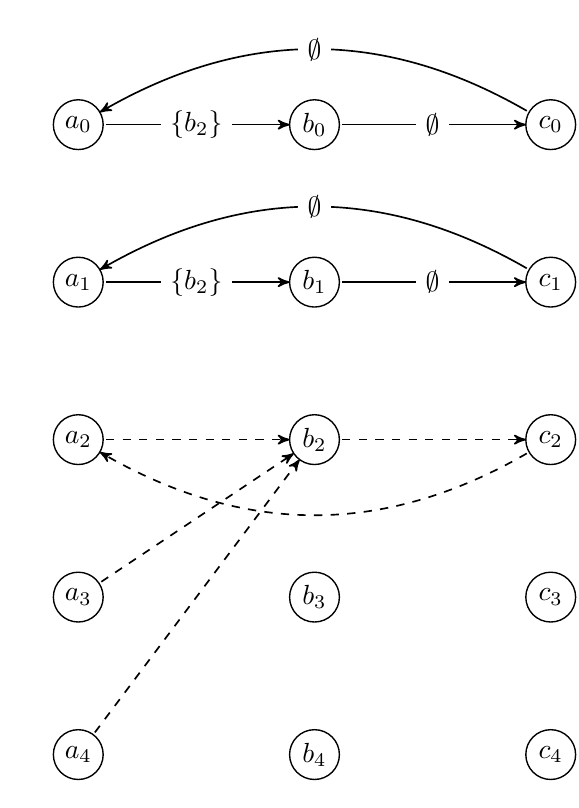
\begin{tikzpicture}
\Vertex[x=0,y=6,L=$a_0$]{a0}
\Vertex[x=3,y=6,L=$b_0$] {b0}
\Vertex[x=6,y=6,L=$c_0$]{c0}

\Vertex[x=0,y=4,L=$a_1$]{a1}
\Vertex[x=3,y=4,L=$b_1$] {b1}
\Vertex[x=6,y=4,L=$c_1$]{c1}



\Vertex[x=0,y=2,L=$a_2$]{a2}
\Vertex[x=3,y=2,L=$b_2$] {b2}
\Vertex[x=6,y=2,L=$c_2$]{c2}

\Vertex[x=0,y=0,L=$a_3$]{a3}
\Vertex[x=3,y=0,L=$b_3$] {b3}
\Vertex[x=6,y=0,L=$c_3$]{c3}

\Vertex[x=0,y=-2,L=$a_4$]{a4}
\Vertex[x=3,y=-2,L=$b_4$] {b4}
\Vertex[x=6,y=-2,L=$c_4$]{c4}

\tikzstyle{EdgeStyle}=[post]

\Edge[label=$\{b_2\}$](a0)(b0)
\Edge[label=$\emptyset$](b0)(c0)

\Edge[label=$\{b_2\}$](a1)(b1)
\Edge[label=$\emptyset$](b1)(c1)

\tikzstyle{EdgeStyle}=[post,bend right]
\Edge[label=$\emptyset$](c0)(a0)
\Edge[label=$\emptyset$](c1)(a1)

\tikzstyle{EdgeStyle}=[dashed,post]
\Edge[](a2)(b2)
\Edge[](a3)(b2)
\Edge[](a4)(b2)
\Edge[](b2)(c2)
\tikzstyle{EdgeStyle}=[dashed,post,bend left]

\Edge[](c2)(a2)
\end{tikzpicture}
\caption{Visualizing lemma \ref{lemma:partial-match}}
\small
\begin{flushleft}
Solid arcs indicate matching $M$, and are labelled vertices tail of arc prefers to their match. Dashed arcs indicate first choice of tail vertex outside $V(M)$.
\end{flushleft}
\end{figure}

\begin{proof}
Let $G' = G[V(G)\backslash V(M)]$ be the subgraph of $G$ induced by vertices unmatched in $M$. Let $c = f(G',b,1)$ and $a = f(G',c,1)$. By our hypothesis, $b = f(G',a,1)$. Let $T = \{abc\}$. Consider the matching $M' = M \cup T$. We will show that $V(M') \cap \cD(G, M') = \emptyset$ to invoke lemma \ref{lemma:inductive} to complete the proof.
\paragraph{}
Let $v \in V(M')$. First consider the case where $v \in V(M) \cap ( B \cup C)$. Since $v \not\in \cD(G,M)$ and $M \subseteq M'$, we have that $v \not\in \cD(G,M')$. Second consider the case where $v \in \{a,b\}$. If $w >_v M'(v)=T(v)$ then $w \in V(M) \cap (B \cup C)$ by our construction of $T$. Since such $ w\not\in \cD(G,M')$ we have $v \not\in \cD(G,M')$. Third consider the case where $v \in V(M) \cap A$. By our hypothesis if $w >_v M'(v) = M(v)$ then $w = b$. Since $b \not\in \cD(G,M')$ we have $v \not\in \cD(G,M')$. Finally consider the case where $v = c$. Since $v \in T$, by our construction of $T$, if $w >_v M'(v)$ then $w \in V(M) \cap A$. Since such $w \not\in \cD(G,M')$ we have $v \not\in \cD(G,M')$. Therefore $V(M') \cap \cD(G,M') = \emptyset$, and since $T \subseteq M'$,  we have $M' \neq \emptyset$ so we may apply lemma \ref{lemma:inductive} to conclude that $G$ has a stable matching.
\end{proof}
\begin{lemma}\label{lemma:partial-match-2}
Let $G=(A\cup B \cup C, E)$ be the hypergraph underlying an instance of $C3GSM$ of size $n$. Let $M$ be a matching in $G$ such that $|M| \geq n-3$. Suppose that 
$$V(M) \cap C \cap \cD(G,M) = \emptyset$$
and there exists $b \in B \backslash V(M)$ satisfying
$$\cD(G,M,V(M) \cap A) = \{b\}$$
and for all $a \in A \backslash V(M)$, $f(G[V(G)\backslash V(M)], a, 1) = b$. Suppose also that there exists $c \in C \backslash V(M)$ satisfying
$$\cD(G,M,V(M) \cap B ) = \{c\}.$$ 
Then $G$ has a stable matching.
\end{lemma}
\begin{proof}
Let $G' = G[V(G)\backslash V(M)]$ be the subgraph of $G$ induced by vertices unmatched in $M$. Let $c' = f(G',b,1)$ be the first choice of $b$ among unmatched vertices in $M$. We consider two cases: when $c' = c$ and when $c' \neq c$.

\paragraph{} First consider when $c' = c$.  Let $a' = f(G',c', 1)$ be the first choice of $c'$ unmatched in $M$. Let $T = \{a'bc\}$. Let $M' = M \cup T$. We will show $V(M') \cap \cD(G,M') =\emptyset$. Let $v \in V(M')$. We give the following case analysis on $v$:
\begin{itemize} 
\item If $v \in V(M) \cap C$ then $v \not\in \cD(G,M')$ since $M \subseteq M'$.
\item If $v = b$ then $w >_v M'(v) = c$ implies $w \in V(M') \cap C$ by our construction of $T$. Thus $w \not\in \cD(G,M')$ and so $v \not\in \cD(G,M')$.
\item If $v \in V(M) \cap A$ then $w >_v M'(v) = M(v)$ implies $w = b$ by our hypothesis. Since $b \not\in \cD(G,M')$ we thus have $v \not\in \cD(G,M')$. 
\item If $v = c$ then $w>_v M'(v) = T(v)$ implies $w \in V(M') \cap A$ and thus $w \not\in \cD(G,M')$, so $v\not\in \cD(G,M')$.
\item If $v \in V(M) \cap B$ then $w>_v M'(v)=M(v)$ implies $w = c$ and thus $w \not\in \cD(G,M')$, so $v \not\in \cD(G,M')$.
\item If $v = a'$ then $w >_v M'(v) = T(v)$ implies that $w \in V(M') \cap B$ by our construction of $T$. Thus $w\not\in \cD(G,M')$ and so $v\not\in \cD(G,M')$. 
\end{itemize}
Therefore $V(M') \cap \cD(G,M') = \emptyset$. Let $S$ be an arbitrary perfect matching in $G$ such that $M' \subseteq S$. Since $|M'| \geq n-2$, $|S\backslash M'| \leq 2$. Since $V(M') \cap \cD(G,M')$ any blocking triple against $S$ must use one vertex from each of three edges in $S\backslash M'$, but since $|S\backslash M'| \leq 2$ this implies it is impossible to form a blocking triple against $S$.
\paragraph{}
Now consider the case when $c' \neq c$. Let $a = f(G',c,1)$. Let $a' = f(G'[V(G')\backslash a], c',1)$ be the first choice of $c'$ among vertices unmatched in $M$ and excluding $c$'s first choice, $a$. Let $b' = f(G'[V(G')\backslash b], a, 1)$. Let $T = \{ab'c\}$ and $T' = \{a'bc'\}$. Form the matching $M' = M \cup T \cup T'$. Again we study $V(M') \cap \cD(G,M')$. Let $v \in V(M')$. In the same manner as the analysis for the previous case, we observe $V(M) \cap C \cap \cD(G,M') = \emptyset$, $b \not \in \cD(G,M')$, $V(M) \cap C \cap \cD(G,M') = \emptyset $, $c\not\in \cD(G,M')$, and $V(M) \cap B \cap \cD(G,M') = \emptyset$, and $a' \not\in \cD(G,M')$. So it remains to consider $v \in \{a, b', c'\}$:
\begin{itemize}
\item If $v = a$ then $w>_a M'(a) = b'$ implies that $w \in V(M) \cap B$ or $w = b$. In either case $w$ is not in $\cD(G,M')$ and thus $v \not\in \cD(G,M')$.
\item If $v = c'$ then $w>_{c'} M'(c') = a$ implies that $w \in V(M) \cap A$ or $w = a$. In either case $w$ is not in $\cD(G,M')$ and thus $v \not\in \cD(G,M')$.
\end{itemize}
Now we did not explicitly choose the partner of $b'$ based on her preference, so we cannot perform the above line of reasoning to conclude that $b' \not\in \cD(G,M')$. Therefore $V(M') \cap \cD(G,M') \subseteq \{b'\}$. Let $S$ be an arbitrary perfect matching of $G$ such that $M' \subseteq S$. Since $|M'| \geq n-1$ and $V(M') \cap \cD(G,M')$ there is exactly  one triple $e \in S \backslash M'$, and the vertex $b'$ from which any blocking triple against $S$ in $G$ could draw its vertices. This is insufficient to form a blocking triple and thus $S$ is a stable matching in $G$.
\end{proof}

\paragraph{}
Just as we did with lemma \ref{lemma:inductive} and lemma \ref{lemma:partialstab}, in lemmas \ref{lemma:partial-match} and \ref{lemma:partial-match-2} we want to replace conditions regarding the set of vertices in blocking triples with ones easier to check in our computer search. The following lemmas do so in a manner analogous to our approach to transforming lemma \ref{lemma:inductive} into lemma \ref{lemma:partialstab}.

\begin{lemma}\label{lemma:comp-match}
Let $G=(A\cup B \cup C, E)$ be the hypergraph underlying an instance of $C3GSM$ of size $n$ where $n-1$ is the best known size satisfying conjecture \ref{conj:stab}. Let $M$ be a matching in $G$. Suppose that $\cB(G[V(M)], M) = \emptyset$, and 
$$ \cS(G,M) \cap (A \cup C) \subseteq V(M)$$
and that there exists $b \in B\backslash V(M)$ satisfying
$$\cS(G,M)\cap B \subseteq \{b\} \cup V(M)$$
and for all $a \in A \backslash V(M)$, $f(G[V(G)\backslash V(M)], a, 1) = b$. Then $G$ has a stable matching.
\end{lemma}

\begin{proof}
Similarly to the proof of lemma \ref{lemma:partialstab} the conditions $$\cB(G[V(M)], M) = \emptyset$$ and $$\cS(G,M) \cap (A \cup C) \subseteq V(M)$$ imply that $$V(M) \cap (B\cup C) \cap \cD(G,M) = \emptyset.$$ Further $$\cS(G,M) \cap B \subseteq \{b\} \cup V(M)$$ implies similarly that $$\cD(G, M, V(M) \cap A) = \{b\}.$$ Thus by lemma \ref{lemma:partial-match} $G$ has a stable matching.
\end{proof}

\begin{lemma}\label{lemma:comp-match-2}
Let $G=(A\cup B \cup C, E)$ be the hypergraph underlying an instance of $C3GSM$ of size $n$. Let $M$ be a matching in $G$ such that $|M| \geq n-3$. Suppose that $\cB(G[V(M)],M) = \emptyset$, and
$$\cS(G,M) \cap A \subseteq V(M)$$
and there exists $b \in B \backslash V(M)$ satisfying
$$\cS(G,M) \cap B \subseteq \{b\} \cup V(M)$$
and for all $a \in A \backslash V(M)$, $f(G[V(G)\backslash V(M)], a, 1) = b$. Suppose also that there exists $c \in C \backslash V(M)$ satisfying
$$\cS(G,M) \cap C \subseteq \{c\} \cup V(M).$$ 
Then $G$ has a stable matching.
\end{lemma}
\begin{proof}
Similar to the proof of \ref{lemma:comp-match}.
\end{proof}

\paragraph{}
Another idea in finding stable matchings is to consider vertices left out of matchings. The following lemma shows that if you have a large enough matching where a dissatisfied vertex is not matched to their last choice then that matching can be extended to a stable matching. 

\begin{lemma}\label{lemma:fixing}
Let $G = (A\cup B \cup C, E)$ be the hypergraph underlying an instance of $C3GSM$ of size $n$. Let $M$ be a matching in $G$ with $\size{M} = n-2$. Suppose there exists $a \in A \cap V(M)$ such that $$V(M) \cap \cD(G,M) = \{a\}.$$ If $f(G, a, $n$)$ is not in $V(M)$ then $G$ has a stable matching.
\end{lemma}
\paragraph{}
In figure \ref{figure:fixing} we see that vertex $a_2$ is the only vertex in $V(M)$ blocking the matching. It prefers only $b_3$ to its partner and $b_4$ is the last choice of $a2$. Since $b_4$ is unmatched in $M$ and $\size(M) = 3 = 5 - 2$ we see that this example satisfies the conditions of lemma \ref{lemma:fixing}.
\begin{figure}[h]\label{figure:fixing}
\centering
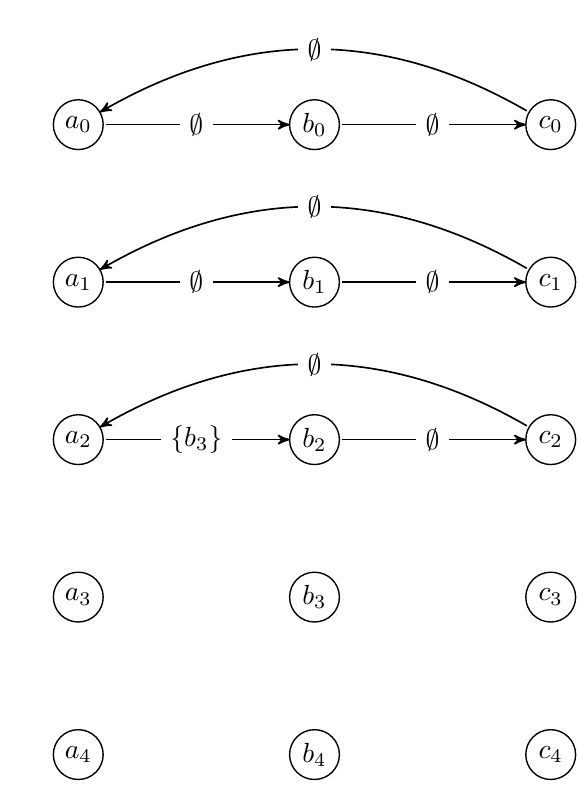
\begin{tikzpicture}
\Vertex[x=0,y=6,L=$a_0$]{a0}
\Vertex[x=3,y=6,L=$b_0$] {b0}
\Vertex[x=6,y=6,L=$c_0$]{c0}

\Vertex[x=0,y=4,L=$a_1$]{a1}
\Vertex[x=3,y=4,L=$b_1$] {b1}
\Vertex[x=6,y=4,L=$c_1$]{c1}



\Vertex[x=0,y=2,L=$a_2$]{a2}
\Vertex[x=3,y=2,L=$b_2$] {b2}
\Vertex[x=6,y=2,L=$c_2$]{c2}

\Vertex[x=0,y=0,L=$a_3$]{a3}
\Vertex[x=3,y=0,L=$b_3$] {b3}
\Vertex[x=6,y=0,L=$c_3$]{c3}

\Vertex[x=0,y=-2,L=$a_4$]{a4}
\Vertex[x=3,y=-2,L=$b_4$] {b4}
\Vertex[x=6,y=-2,L=$c_4$]{c4}

\tikzstyle{EdgeStyle}=[post]

\Edge[label=$\emptyset$](a0)(b0)
\Edge[label=$\emptyset$](b0)(c0)

\Edge[label=$\emptyset$](a1)(b1)
\Edge[label=$\emptyset$](b1)(c1)

\Edge[label=$\{b_3\}$](a2)(b2)
\Edge[label=$\emptyset$](b2)(c2)

\tikzstyle{EdgeStyle}=[post,bend right]
\Edge[label=$\emptyset$](c0)(a0)
\Edge[label=$\emptyset$](c1)(a1)
\Edge[label=$\emptyset$](c2)(a2)

\end{tikzpicture}
\caption{Visualizing lemma \ref{lemma:fixing}}
\small
\begin{flushleft}
Solid arcs indicate matching $M$, and are labelled with $\cD(G,M,\{t\})$ where $t$ is the tail vertex of the arc. In this figure $b_4$ is the last choice of $a_2$.
\end{flushleft}
\end{figure}
\paragraph{}
\begin{proof}
By the size of $M$ there exists $b,b' \in B$ such that $\{b,b'\} = B \backslash V(M)$. Without loss say that $b = f(G, a, n)$. Let $G' = G[V(G)\backslash V(M)]$ and let $c' = f(G',b', 1)$. Let $a' \in A\backslash V(M)$. Let $T = \{a'b'c'\}$ and let $T' = \{a''bc''\}$ where $a''$ and $c''$ the remaining two vertices unmatched in $M$ or $T$. Then $S = M \cup T \cup T'$ is a perfect matching of $G$. We claim that $S$ is stable.
\paragraph{}
Let $v \in V(G)$. We will show that $v \not\in \cD(G,S)$ and thus that $S$ is stable. If $v \in V(M) \cap (A\backslash \{a\} \cup B \cup B)$ then $v \not\in \cD(G,M)$ and thus $v \not \in \cD(G,S)$ as $M \subseteq M$. If $v = b'$ then $w >_v S(v)$ implies that $w \in V(M) \cap C$ by our construction of $T$. Since such $w \not\in \cD(G,S)$ we have $v=b' \not\in \cD(G,S)$. Now if $v = a$ then if $w>_v S(v)$ then $w \in V(M) \cap B$ or $w = b'$. In either case $w \not\in \cD(G,S)$ and thus $a \not \in \cD(G,S)$. Now we have $V(M) \cap A \cap \cD(G,S) = \emptyset$. So $\cD(G,S) \subseteq \{a',a'',b, c',c''\}$. But $\{a',a'',b, c',c''\}$ consists only of vertices matched together in either the triple of $T$ or the triple of $T'$, hence they cannot form a blocking triple, as any triple from $\{a',a'',b, c',c''\}$ would contain a vertex and their match in $S$. Therefore $\cD(G,S) = \emptyset$ and thus $S$ is stable.
\end{proof}

\paragraph{Stabilizing $A,B,C$:}
The previous lemmas have the common theme of building matchings that have no blocking triples in the hypergraph among the matched vertices then using induction to make the matching perfect. The following lemma and corollary take a different strategy. Whereas before we tried to create a matching where matched vertices have no blocking triples even with unmatched vertices, alternatively we can attempt to pair all the vertices in one of $A,B,C$ with a partner in such a way that none of them will participate in a blocking triple.
\paragraph{}
A motivation to consider this different approach comes from the context we intend to use these lemmas. In our computer search procedure to be defined in \ref{sec:computersearch} we use these lemmas to eliminate instances of $C3GSM$ from consideration without actually finding a stable matching. A desirable feature in these lemmas is that they can eliminate instances with minimal knowledge of vertices preferences. That is a lemma that can prove a stable matching exists only considering $f(G,v,1)$ for all $v$ is preferable to one that also needs to check $f(G,v,2)$.
\paragraph{}
With the above motivation in mind, the intuitive difference between the lemmas previously described and those to be described is that the previous lemmas capture a lot of instances where vertices of $A$ or $B$ or $C$ largely agree on which vertices are high ranking in terms of preferences. For example when there is a $1,1,1$ triple corollary \ref{cor:1cycle} proves the existence of a stable matching. A distinctly difference situation, but still operating within the first choices of vertices occurs when there are no $1,1,1$ triples, but each vertex in $A$ has a different first choice vertex in $B$. Then one of the corollaries to follow, corollary \ref{cor:alldiff}, says that there is a stable matching in this instance.
\begin{lemma}\label{lemma:genderstab}
Let $G=(A\cup B\cup C, E)$ be the hypergraph underlying an instance of $C3GSM$. Let $M$ be a perfect $A$-$B$ matching (that is a perfect matching of the underlying complete bipartite graph between $A$ and $B$). Let $B' = \{ b \in B : \exists a \in A : b >_a M(a) \}$. Hence $B'$ is the set of vertices through which agents of $A$ can form blocking triples. If for all $b, b' \in B'$, $f(G,b,1) \neq f(G,b',1)$ then $G$ has a stable matching.
\end{lemma}
\begin{figure}[h]
\centering
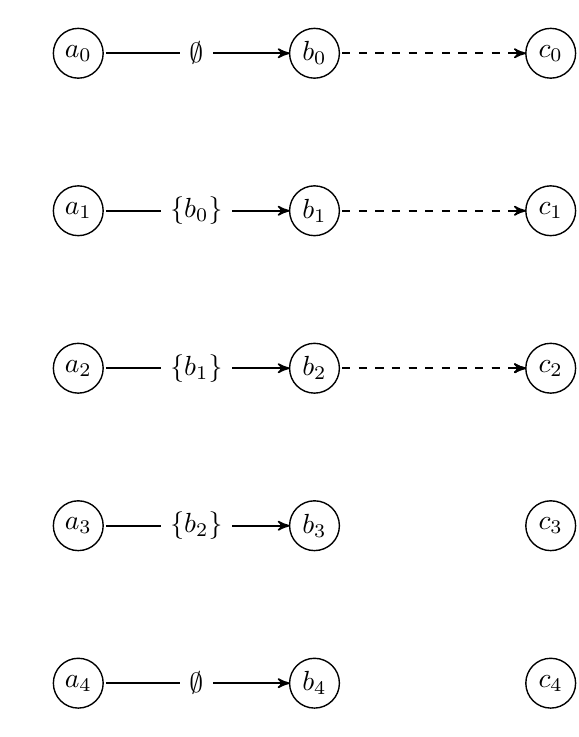
\begin{tikzpicture}
\Vertex[x=0,y=6,L=$a_0$]{a0}
\Vertex[x=3,y=6,L=$b_0$] {b0}
\Vertex[x=6,y=6,L=$c_0$]{c0}

\Vertex[x=0,y=4,L=$a_1$]{a1}
\Vertex[x=3,y=4,L=$b_1$] {b1}
\Vertex[x=6,y=4,L=$c_1$]{c1}



\Vertex[x=0,y=2,L=$a_2$]{a2}
\Vertex[x=3,y=2,L=$b_2$] {b2}
\Vertex[x=6,y=2,L=$c_2$]{c2}

\Vertex[x=0,y=0,L=$a_3$]{a3}
\Vertex[x=3,y=0,L=$b_3$] {b3}
\Vertex[x=6,y=0,L=$c_3$]{c3}

\Vertex[x=0,y=-2,L=$a_4$]{a4}
\Vertex[x=3,y=-2,L=$b_4$] {b4}
\Vertex[x=6,y=-2,L=$c_4$]{c4}

\tikzstyle{EdgeStyle}=[post]

\Edge[label=$\emptyset$](a0)(b0)
\Edge[label=$\{b_0\}$](a1)(b1)
\Edge[label=$\{b_1\}$](a2)(b2)
\Edge[label=$\{b_2\}$](a3)(b3)
\Edge[label=$\emptyset$](a4)(b4)



\tikzstyle{EdgeStyle}=[dashed,post]
\Edge[](b0)(c0)
\Edge[](b1)(c1)
\Edge[](b2)(c2)

\Edge[](b2)(c2)

\end{tikzpicture}
\caption{Visualizing lemma \ref{lemma:genderstab}}
\small
\begin{flushleft}
Solid arcs indicate matching $M$, and are labelled with $\cD(G,M,\{t\})$ where $t$ is the tail vertex of the arc. Dashed arcs indicate first choice of tail vertex.
\end{flushleft}
\end{figure}
\begin{proof}
Let $C' = \{ c \in C : \exists b\in B', c = f(G,b,1)\}$. Since $f(G,\cdot,1)$ is a bijection between $B'$ and $C'$ we can form the matching $S_1 = \{abc \in E: a = M(b)\text{ and } c = f(G,b,1)\}$. Let $S_2$ be an arbitrary perfect matching of $G[V(G) \backslash V(S_1)]$, the remaining vertices unmatched in $S_1$. Let $S = S_1 \cup S_2$. Then $S$ is a complete matching on $G$. We claim that $S$ is stable. Suppose for a contradiction there exists blocking triple $a,b,c$. Then $b >_a M(a)$ and hence $b \in B'$. Thus $M(b) = f(G,b,1)$ and so $M(b) \geq_b c$ by definition of $f(G,\cdot,1)$, but this contradicts that $a,b,c$ is a blocking triple since that requires $c >_b M(b)$.
\end{proof}
\begin{corollary}\label{cor:alldiff}
If $f(G,a,1) \neq f(G,a',1)$ for all $a,a' \in A$ in a hypergraph $G=(A\cup B \cup C, E)$ underlying a $C3GSM$ instance then $G$ has a stable matching.
\end{corollary}
\begin{proof}
Observe that $M = \{ab : b = f(G,a,1)\}$ is a perfect $A$-$B$ matching since $f(G,\cdot, 1)$ is a bijection between $A$ and $B$. In this case we have $B' = \emptyset$ by the definition of $f(G,\cdot,1)$. Thus we may invoke lemma \ref{lemma:genderstab} to obtain a stable matching of $G$.
\end{proof}
\subsection{Symmetry in Problem Instances}\label{subsec:symmetry}
\paragraph{}
We will now turn our attention towards formulating an equivalence relation on instances of $C3GSM$. In doing so we hope to answer the question ``when does knowledge that one instance of $C3GSM$ has a stable matching translate to knowing that another instance does?". This question is motivated by our efforts to design a computer search protocol in the next subsection. In checking if all $C3GSM$ instances of a certain size have a stable matching it is desirable to avoid repeated work by not checking instances ``symmetric" to one already checked.

\paragraph{}Let $G$ and $H$ be two hypergraphs underlying distinct instances of $C3GSM$. Let $>_v$ for $v\in V(G)$ denote the orders associated with vertices in $G$. Let $>'_v$ for $v \in V(H)$ denote the orders associated with vertices in $H$. We say that $G$ and $H$ are {\it equivalent} in the sense that they denote symmetric problem instances, written $G \equiv H$ if there exists a bijection $\phi: V(G) \rightarrow V(H)$ such that for all $v \in V(G)$,
 \begin{equation}\label{cond:order}
 w >_v u \text{ if and only if } \phi(w) >'_{\phi(v)} \phi(u).
 \end{equation}
 
\begin{note}
It is clear that $\equiv$ is an equivalence relation. Through the identity bijection we have reflexivity, through the inverse bijection we have symmetry, and through composition of bijections we have transitivity. Thus $\equiv$ is an equivalence relation as desired.
\end{note}
 \begin{lemma}\label{lemma:equiv}
 If $G \equiv H$ then $G$ has a stable matching if and only if $H$ has a stable matching
 \end{lemma}
 \begin{proof}
 \paragraph{}
 By symmetry it suffices to prove the sufficiency direction. Let $M$ be a stable matching of $G$. Define the matching $\phi(M)$ in $H$ as
 $$\phi(M) = \{ \phi(a)\phi(b)\phi(c): abc \in M \}.$$
 It is not hard to see that since $M$ is a matching and $\phi$ is a bijection that $\phi(M)$ is a matching. Suppose for a contradiction that $\phi(M)$ is not stable for $H$. Let $xyz$ be a blocking triple of $\phi(M)$ against $H$. Let $abc = \phi^{-1}(x)\phi^{-1}(y)\phi^{-1}(z)$. By our definition of $\phi(M)$, $abc \not\in M$. Further since $y >_x \phi(M)(x)$, by the definition of $\phi$ we have $b >_a M(a)$. Similarly $c>_b M(b)$ and $a>_c M(c)$. Thus $abc$ is a blocking triple of $M$, a contradiction.
 \end{proof}
 \begin{note}\label{note:labels}
 Since we require that $\phi$ is a bijection it is necessary that $G$ and $H$ underly instances of $C3GSM$ of the same size, say $n$. Let $V(G)$ be partitioned as $V(G)_0 \cup V(G)_1 \cup V(G)_2$ since $G$ is tripartite. Let $i \in \{0,1,2\}$. Since each $V(G)_i$ is of size $n$ we may label the elements of $V(G)_i$ as $(i,0), \dots, (i,n-1)$. We may use the same labelling convention for $V(H)$. Then $\phi$ is a bijection from $Z_3 \times Z_n$ to itself which preserves each vertex's order of its neighbours (and consequently the graph incidence structure). So we can say a few things about $\phi$ from this perspective.
 \end{note}
 \paragraph{Observations} Firstly by $\ref{cond:order}$ we must preserve the graph structure. Hence for any $i \in \{0,1,2\}$ there exists $j \in \{0,1, 2\}$ such that $\phi(V_i) = V_j$ otherwise the graph $H$ is not tripartite. Furthermore if $\phi(V_i) = V_j$ then $\phi(V_{i+1}) = V_{j+1}$ with addition taken modulo $3$. Again this follows from condition \ref{cond:order}.
\paragraph{}
Together the previous observations imply that there exists $r \in \{0,1,2\}$ such that $\phi(V_i) = V_{i+r}$ for any $i \in\{0,1,2\}$. Hence we can specify $\phi$ by $(r,\Pi)$ where $\Pi = \{\pi_0, \pi_1,\pi_2\}$ is a family of three permutations $\pi_i$ on $\Z_5$, one for each part $V(G)_i$. In specifying $\phi=(r,\Pi)$ we require that $(r,\Pi)$ satisfying a translation of condition \ref{cond:order} for all $(i,a) \in V(G)$; that is, 
\begin{equation}\label{cond:orderT}
(i+1,b) >_{(i,a)} (i+1, b') \text{ if and only if } (i+1+r, \pi_{i+1}(b)) >_{(i+r,\pi_i(a))} (i+1+r, \pi_{i+1}(b')).
\end{equation}
\paragraph{}
Of interest to us are the equivalence classes of a given problem instance under $\equiv$. For a hypergraph $G$ underlying an instance of $C3GSM$ we will denote the equivalence class containing $G$ by $[G]$. In a procedure to test whether instances of $C3GSM$ of a certain size have stable matchings one can hope to avoid unnecessary repeated work by only testing one representative from $[G]$ instead of all instances in $[G]$. We will now define a strict total order on instances of $C3GSM$ of size $n$, with the goal of obtaining a method to test only the minimum element with respect to this order for each equivalence class $[G]$.
\paragraph{}
To define an order on instances of $C3GSM$ of size $n$ we will translate instances into finite sequences then apply a natural lexicographic order to said sequences. The next sequence of definitions will make this formal.

\paragraph{}Let $G$ be a hypergraph underlying an instance of $C3GSM$ of size $n$. Let $i \in \{0,1,2\}$ and let $j \in \{0,\dots,n-1\}$. We define
$$seq(G,i,j) = f(G,(i,j),1)f(G,(i,j),2)\dots f(G,(i,j),n)$$
to be the sequence of first through to last choices for vertex $(i,j)$.We sometimes will refer to $seq(G,i,j)$ as $(i,j)$'s preference list.

\paragraph{}Let $G$ be a hypergraph underlying an instance of $C3GSM$ of size $n$. Let $i \in \{0,1,2\}$. We define a sequence for each vertex partition, $seq(G,i)$, by appending $seq(G,i,j)$ for each $j \in \{0, \dots, n-1\}$.  Formally we say
$$seq(G, i) = seq(G,i,0)\dots seq(G,i,n-1).$$

\paragraph{}Let $G$ be a hypergraph underlying an instance of $C3GSM$ of size $n$. We define our sequence for $G$, $seq(G)$ by appending the sequences corresponding to each vertex partition. Formally we have
$$seq(G) = seq(G,0)seq(G,1)seq(G,2).$$
So $seq(G)$ consists of appending the preference lists of vertices $0$ through $n-1$ of $V(G)_0$ followed by appending the same for $V(G)_1$ and finally $V(G)_2$.

\paragraph{}We will use the symbol $>_{lex}$ to denote our lexicographical order of instances of $C3GSM$ of a given size $n$. Let $G$ and $H$ be hypergraphs underlying size $n$ instances of $C3GSM$. We say $G >_{lex} H$ if $seq(G)$ is lexicographically larger than $seq(H)$. That is there exists some $k$ such that
$$seq(G)_k > seq(H)_k$$
and for all $i < k$
$$seq(G)_i = seq(H)_i.$$
We compare vertices in $seq(G)_k$ and $ seq(H)_k$ as if they are natural numbers corresponding to their labels. That is if $seq(G)_k = (i,a)$ and $seq(H)_k = (j,b)$ then we simply say $seq(G)_k > seq(H)_k$ if and only if $a>b$. 

\paragraph{}
Unfortunately we do not have a full characterization of the lexicographic minimum of a given equivalence class under the order $>_{lex}$, which would be desirable. Instead we do have some necessary conditions which we collect in the following lemma. These are useful for finding instances of $C3GSM$ that we can avoid testing in a computer search since we are certain we are at least testing the lexicographic minimum of each equivalence class.
\paragraph{}
The following lemma presents four necessary conditions which we will summarize intuitively before presenting in rigorous formality. The first condition says that vertex $(0,0)$ has preference list $0,1,\dots, n-1$, which means that $(1,0) >_{(0,0)} (1,1) >_{(0,0)} (1,2) >_{(0,0)}\dots >_{(0,0)} (1,n-1).$ The second condition says the same thing regarding $(1,0)$. The third condition says that preference lists of vertices in $A$ are sorted lexicographically. The last condition says that you cannot rotate the roles of $A,B,C$ to obtain a lexicographically smaller instance than the lexicographic minimum.
\begin{lemma}\label{lemma:nec-symmetry}
Let $G$ be the hypergraph underlying an instance of $C3GSM$ of size $n$. If $G$ is the lexicographic minimum of $[G]$ then the following are satisfied:
\begin{enumerate}
\item $seq(G,0,0) = 0,1,\dots,n-1$,
\item $seq(G,1,0) = 0,1,\dots,n-1$,
\item let $a, b \in \{0,1,\dots, n-1\}$ and let $k \in \{1,\dots,n\}$. If $f(G,(0,a), k) < f(G,(0,b), k)$ and for all $j \in [0,k) \cap \Z$, $f(G,(0,a),j) =f(G,(0,b),k)$ then $a < b$,
\item We have that $$seq(G) \leq_{lex} seq(G,1)seq(G,2)seq(G,0)$$ and $$seq(G) \leq_{lex} seq(G,2)seq(G,0)seq(G,1).$$
\end{enumerate}
\end{lemma}
\begin{proof}
We first prove $(1)$. Let $\phi : V(G) \rightarrow V(G)$ be described by $(0,e,\pi_1, e)$ where $e$ denotes the identity permutation and $\pi_1$ is the permutation which sends $seq(G,0,0)$ to $0,1,\dots,n-1$. Let $H$ be the hypergraph underlying an instance of $C3GSM$ such that $G \equiv H$ with respect to $\phi$. Since $G$ is the lexicographic minimum of $[G]$ and $H \in [G]$, $seq(G,0,0) \leq_{lex} seq(H,0,0) = 0,1,\dots,n-1$. Since $0,1,\dots,n-1$ is the lexicographic minimum sequence possible we have $seq(G,0,0) = 0,1,\dots,n-1$.
\paragraph{}
To prove $(2)$ we do something similar to $(1)$. Let $\phi$ be described by $(0,e,e,\pi_2)$ where $\pi_2$ is the permutation which sends $seq(G,1,0)$ to $0,1,\dots,n-1$. Let $H$ be the hypergraph underlying an instance of $C3GSM$ such that $G \equiv H$ with respect to $\phi$. Observe that since $r = 0$ and $\pi_0 = \pi_1 = e$, $seq(G,0) = seq(H,0)$. Since $G$ is the lexicographic minimum of $[G]$ and $H \in [G]$, $seq(G,1,0) \leq_{lex} seq(H,1,0) = 0,1,\dots,n-1$. Since $0,1,\dots,n-1$ is the lexicographic minimum sequence possible we have $seq(G,1,0) = 0,1,\dots,n-1$.
\paragraph{}
We now turn our attention to proving $(3)$. Observe that $seq(G,0,a) <_{lex} seq(G,0,b)$. Let $\phi$ be described by $(0,\pi_0,e,e)$ where $\pi_0$ which transposes $a$ and $b$. Let $H$ be the hypergraph underlying an instance of $C3GSM$ such that $G \equiv H$ with respect to $\phi$. Suppose for a contradiction that $b<a$. Since $r=0$, $\pi_1=\pi_2=e$, and $\pi_0$ simply transposes $a$ and $b$, this yields 
\begin{align*}seq(H,0) &= seq(G,0,0) \dots seq(G,0,b-1)seq(G,0,a)seq(G,0,b+1)\\
&\dots seq(G,0,a-1) seq(G,0,b) seq(G,0,a+1) \dots seq(G,0,n-1) \\
&<_{lex} seq(G,0).\end{align*}
This contradicts the lexicographic minimality of $G$.
\paragraph{}
Finally we prove $(4)$. Let $\phi$ be described by $(1,e,e,e)$. We will prove $seq(G)$ is lexicographically at most $seq(G,1)seq(G,2)seq(G,0)$. The proof that $G$ is lexicographically smaller that $seq(G,2)seq(G,0)seq(G,1)$ follows similarly using $(2,e,e,e)$. Let $H$ be the hypergraph underlying an instance of $C3GSM$ such that $G \equiv H$ with respect to $\phi$. Since $\pi_0=\pi_1=\pi_2=e$ and $r=1$ we have that
$$seq(H) = seq(G,1)seq(G,2)seq(G,0)$$
and thus by the lexicographic minimality of $G$, $seq(G) \leq_{lex} seq(H)$ and the result follows.
\end{proof}
\subsection{Computer Search}\label{sec:computersearch}
\paragraph{}
Our goal now is to describe a computer search procedure to test all instances of $C3GSM$ for a given size $n$ under the assumption that for $k<n$ it is known that all instances of $C3GSM$ have a stable matching. In our case we study $n=5$. A major challenge towards solving this problem computationally is that enumerating all instances of $C3GSM$ would be infeasible. For each vertex there is one possible preference order or each permutation of $\{1,\dots,n\}$. There are $3n$ such vertices, and thus there are $(5!)^{15}$ possible problem instances for $C3GSM$ with size $5$. 
\paragraph{}
We resolve to overcome the sheer number of possible $C3GSM$ instances by eliminating instances from consideration using our symmetry and sufficiency checks theory from the previous subsections. Our approach is based on the idea that if we relax the total orders to partial orders giving only the first few preferences of each vertex and can find a perfect stable matching then any $C3GSM$ instance that results from completing the partial order will also have said stable matching. The following theory formalizes this idea. Herein and henceforth we use the ordered pair labeling for vertices of $G$ as outlined in note \ref{note:labels}.

\paragraph{}A {\it partially} {\it specified} {\it instance} of $C3GSM$ of size $n$ provides a complete $3$-partite hypergraph $G$, as in an instance of $C3GSM$, but not the total orders for each of the vertices of $G$. In our partially specified instance there exists a vertex $(g,v)$ called the {\it extender}, and an integer $\ell \in \{1, \dots, n+1\}$ called the {\it length} satisfying that:
\begin{enumerate}
\item For all $(h,w)$ where $h < g$, or $h=g$ and $w < v$ we have that 
$$f(G, (h,w), 1), \dots, f(G,(h,w),\ell)$$
are specified in the partial order of $(h,w)$, and 
$$f(G, (h,w), \ell+1), \dots, f(G, (h,w), n)$$
are not specified in the partial order of $(h,w)$. That is, $(h,w)$ specifies their top-ranked $\ell$ preferences in their partial order.
\item For all $(h,w)$ where $h = g$ and $w \geq v$, or $h > g$ we have that
$$f(G, (h,w), 1), \dots, f(G, (h,w), \ell -1)$$
are specified in the partial order of $(h,w)$ and
$$f(G, (h,w), \ell), \dots, f(G,(h,w), n)$$
are not specified in the partial order of $(h,w)$. That is, $(h,w)$ specifies their top-ranked $\ell-1$ preferences in their partial order.
\end{enumerate}

\paragraph{}
The idea of the definition is that every vertex lexicographically smaller than the extender has only specified their first $\ell$ choices, where $\ell$ is the length, and every vertex lexicographically at least the extender has only specified their their first $\ell-1$ choices. We give a few quick examples:
\begin{itemize}
\item A partially specified instance of $C3GSM$ with no vertices specifying any of their orders has extender $(0,0)$ and length $1$. This is the unique ``empty" instance.
\item A partially specified instance of $C3GSM$ of size $5$ that is in fact an instance of $C3GSM$ proper has extender $(0,0)$ and length $6$. Observe that since $6$ is one greater than the size of the instance this is the only situation where the length is $6$.
\item The two previous examples can be generalized. A partially specified instance of $C3GSM$ of size $n$ where each vertex has specified their first $k$ choices, for $k \in \{0, \dots, n\}$ has extender $(0,0)$ and length $k+1$.
\item A partially specified instance of $C3GSM$ that has only every vertex of $V(G)_0$ specifying their first choice and no other choices specified has extender $(1,0)$ and length $1$.
\item A partially specified instance of $C3GSM$ of size $5$ with extender $(2,2)$ and length $3$ has every vertex of $V(G)_0$ and $V(G)_1$ specifying their first $3$ choices. It also $(2,0)$ and $(2,1)$ specifying their first $3$ choices. The vertices $(2,2)$, $(2,3)$, and $(2,4)$ specify only their first $2$ choices.
\end{itemize}

\paragraph{}Let $I$ and $I'$ be two partially specified instances of $C3GSM$ of size $n$ with the same underlying hypergraph $G$. Let $(g,v)$ be the extender of $I$ and $\ell$ be the length of $I$. Let $(g',v')$ be the extender of $I'$ and $\ell'$ be the length of $I'$. We say that $I'$ is an {\it extension} of $I$ provided that for all $v \in V(G)$ the preference order specified by $v$ in $I$ is contained in the preference order specified by $v$ in $I'$, and the following cases are satisfied:
\begin{enumerate}
\item If $(g,v) = (2,n-1)$ then $(g',v') = (0,0)$ and $\ell' = \ell + 1$.
\item If $g < 2$ and $v = n-1$ then $(g',v') = (g+1, 0)$ and $\ell' = \ell$.
\item If $g<2$ and $v<n-1$ then $(g',v') = (g, v+1)$ and $\ell' = \ell$.
\end{enumerate}

\paragraph{}
For example consider the partially specified instance of $C3GSM$ of size $5$ where the first four vertices of $V(G)_0$ specify their first choice to be $(1,0)$, and the remaining vertices specify no choices. This instance has extender $(0,4)$ and length $1$. The partially specified instances of $C3GSM$ where the first four vertices of $V(G)_0$ specify their first choice to be $(1,0)$ and the vertex $(0,4)$ specifies $f(G,(0,4),1) = k$ where $k \in \{(1,0), \dots, (1,4)\}$ are extensions of our original partially specified instance. In this example the indicator of our original instance satisfies the third case in our definition of extension. 
\paragraph{}
As another example consider an instance of $C3GSM$ where each vertex has specified their first choice, and each vertex of $V(G)_0$ has specified their second choice. Each extension would have the same preferences but additionally have $(1,0)$ specify their second choice. This example covers the second case in our definition of extension. 
\paragraph{}
Any instance of $C3GSM$ where the first $k$ preferences have been specified for each vertex provides an example for the first case in our definition of extension. In any such instance the extensions have vertex $(0,0)$ specifying their $k+1$-th preference.

\paragraph{}Let $I$ and $I'$ be partially specified instances of $C3GSM$ with the same underlying graph. We say that $I'$ is a {\it descendant} of $I$ if there exists a sequence of partially specified $C3GSM$ instances
$$I = I_0, I_1, \dots, I_k=I'$$
such that for all $i \in \{0,\dots, k-1\}$ we have that $I_{i+1}$ is an extension of $I_i$.

\paragraph{}Let $I$ be a partially specified instance of $C3GSM$. We say that $I$ is {\it stable} if every instance of $C3GSM$ which is a descendant of $I$ has a stable matching.

\paragraph{Computer Search Algorithm}
We now describe our procedure for deciding if each instance of $C3GSM$ of size $n=5$ has a stable matching. For any partially specified instance of $C3GSM$, $I$, let $\cE(I)$ denote the list of partially specified instances of $C3GSM$ which are extensions of $I$ and let $\cP(I)$ denote the unique instance that $I$ is an extension of. For convention we will say $\cP(I) = I$ for the empty instance with extender $(0,0)$ and length $1$. The algorithm is as follows:
\begin{enumerate}
\item Let $I$ be the partially specified instance of $C3GSM$ of size $5$ with extender $(0,0)$ and length $1$.
\item While $\cE(I) \neq \emptyset$ or $\cP(I) \neq I$
	\begin{enumerate}
	\item If $I$ is stable via a lemma of \ref{subsec:sufficient} or the graph underlying $I$ does not satisfy a conclusion of lemma \ref{lemma:nec-symmetry} then set $\cE(I) \leftarrow \emptyset$ and $I \leftarrow \cP(I)$, and continue to the next iteration of step $2$.
	\item Else If $\cE(I) = \emptyset$ then return $I$ as a counterexample to conjecture \ref{conj:stab}
	\item Otherwise let $E \in \cE(I)$. Remove $E$ from $\cE(I)$ and set $I \leftarrow E$. 
	\end{enumerate}
\item If While loop terminates with no counterexample found then conjecture \ref{conj:stab} is proven for $n=5$ and return that it is so.
\end{enumerate}
\paragraph{On using lemmas of subsection \ref{subsec:sufficient}}
In step $2(a)$ it may not be clear how to use the lemmas of subsection \ref{subsec:sufficient} to conclude that $I$ is stable. This is actually easier to verify in many cases than is immediately apparent. If one can form a matching in $I$ that only matches vertices with those that they have specified a ranking for, then it is easy to see which vertices they prefer to the matching. When the $k$-th choice of a vertex in an extension is specified all their choices of rank less than $k$ have previously been specified. Hence if we have a matching $M$ valid in a partially specified instance $I$, by which we mean for each $v \in V(M)$, $M(v)$ is ranked in $v$'s partial order with respect to $I$, then the set of vertices preferred by some $v \in V(M)$ to $M(v)$ is completely known at $I$ and does not change for any descendant of $I$. Therefore Lemmas \ref{lemma:partialstab}, \ref{lemma:comp-match}, \ref{lemma:comp-match-2}, and \ref{lemma:genderstab} can be checked for instance $I$ without worry that any descendant instances would violate their hypotheses. This follows since descendant instances are generated by a sequence of extensions which do not alter the set of vertices preferred by any matched vertex to their partner. There is a notable exception in lemma \ref{lemma:fixing} which we use in a slightly different way.
\paragraph{Fixing Choices With Lemma \ref{lemma:fixing}}
Lemma \ref{lemma:fixing} requires knowledge of a vertex's last choice in order to conclude that the given problem instance has a stable matching. Unfortunately lemmas which rely on last choices don't naturally lend themselves to cutting instances from consideration early on via step $2(a)$. There is an alternative approach to using them though. Suppose there is a partially specified instance $I$ and matching $M$ for which each vertex except for $a$ that is matched in $I$ is matched to a partner that they have already specified their ranking for in $I$, and all vertices $a$ has specified a ranking for are matched in $M$. Also suppose that $M$ satisfies all the requirements of lemma \ref{lemma:fixing} except for the requirement that $a$'s last choice is unmatched in $M$ (as a consequence of not knowing $a$'s last choice). Then by lemma \ref{lemma:fixing} any fully specified instance of $C3GSM$ extended from $I$ wherein $M(a)$ is not the last choice of $a$ is one where $a$'s last choice is unmatched in $M$ and hence has a stable matching. Thus we know we need only consider extensions where $M(a)$ is the last choice of $a$. If one can find another such matching $M'$ with $M'(a) \neq M(a)$ then we know $I$ is stable since the last choice of $a$ cannot simultaneously be $M'(a)$ and $M(a)$.
\paragraph{Example of Fixing Choices}
Consider the following partially specified instance of $C3GSM$:
\begin{align*}
a_0 &: b_0 > b_1  &&b_0: c_0 > c_1 &\ &c_0:a_4 > a_3\\
a_1 &: b_1 > b_0  &&b_1: c_1 > c_0 &\ &c_1: a_0 > a_1 \\
a_2 &: b_0  > b_2  &&b_2: c_2  > c_3 &\ &c_2: a_2 \\
a_3 &: b_0  > b_3  &&b_3: c_0  > c_3 &\ &c_3: a_0\\
a_4 &: b_0  > b_2  &&b_4: c_0  > c_3 &\ &c_4: a_0\\
\end{align*}
If we consider matching $M_1 = \{a_0b_0c_0, a_1b_1c_1, a_2b_2c_3\}$ then the matching is only violated with respect to the partner of $c_0$. Further there are no blocking triples internal to $M_1$ except possibly with $c_0$ and $\size{M_1} = 3 = 5-2$. By the previous discussion the only descendants of this instance which could possibly not be stable are those where $c_0$ has $a_0$ as their last choice. But if we consider $M_2= \{a_0b_1c_1, a_1b_0c_0, a_2b_2c_2\}$ this matching similarly says the only descendants of this instance which could possibly not be stable are those where $c_0$ has $a_1$ as their last choice. Since $c_0$ cannot possibly have both $a_0$ and $a_1$ as their last choice all descendants of this instance are stable.
\paragraph{Correctness of Algorithm}
With the prior discussion in mind it becomes clear that the computer search procedure works. If the graph underlying some partially specified instance $I$ does not satisfy a conclusion of lemma \ref{lemma:nec-symmetry} then no instance of $C3GSM$ which is a descendant of $I$ will satisfy that same conclusion and thus is not the lexicographical minimum instance of its equivalence class. Therefore step $2(a)$ only eliminates instances of $C3GSM$ which not lexicographical minima or have a stable matching by a lemma of subsection \ref{subsec:sufficient}. In the former case, by lemma \ref{lemma:equiv}, we need not consider this instance as it has a stable matching if and only if the lexicographical minimum of its equivalence class, which we do consider, has a stable matching. In the latter case the sufficient condition lemmas tell us directly we need not consider these instances as they have a stable matching. Hence all removed instances during the execution of the computer search algorithm have a stable matching or are equivalent to an instance considered by the algorithm. Furthermore all instances of $C3GSM$ are considered since they all are descendants of the ``empty" instance the algorithm starts running with.
\paragraph{}
The intuition behind our computer search procedure is that we can often conclude that a problem instance has a stable matching without looking at all the preferences of each vertex. Recall, for instance that if there is a cycle of vertices, all respective first choices of each other, then there is a stable matching. The goal is to develop enough theory of lemmas that imply stable matchings as in subsection \ref{subsec:sufficient} that we can eliminate many instances in step $2(a)$ early on in execution. To see the benefit of this suppose we eliminate in step $2(a)$ a partially specified instance that has only specified each vertex's first choice. There are $(4!)^{15}$ possible fully specified instances of $C3GSM$ which are descendants of the eliminated instance that we do not need to check now.
\paragraph{Results of Computational Experiments}
We implemented our computer search algorithm in Java (see \href{https://github.com/tothw/cyclicstablematching}{github.com/tothw/cyclicstablematching} for our source code). We were unsuccessful in getting the algorithm to terminate but we were able to eliminate many preferences. We are confident that our computations are close to proving that all $C3GSM$ instances of size $5$ admit a stable matching or finding a counterexample to \ref{conj:stab}. Our confidence comes from the observation that the current implementation very rarely needs to go deeper than specifying every vertices second choice to decide that the instance has a stable matching. However our computations have not terminated yet, so nothing can be said about the conjecture for $n=5$ at this time. On the other hand for considering instance of size $n \geq 6$ we will need considerably more ideas characterizing when an instance has a stable matching in order to hope that the computational approach will go through.



%======================================================================
%Conclusion
%======================================================================
\chapter{Conclusion}

\paragraph{}
In this chapter we summarize our work and suggest some open problems for further investigation.

\section{Summary}

\paragraph{}
The focus of this thesis has been on understanding the nature of stable matching problems. In Chapter $2$ we gave the necessary background to read this work, and also gave some interesting previously known results about the structure of the classical stable matching problem. This culminated in the lattice theorem for stable matchings \ref{theorem:lattice}. 
\paragraph{}
In Chapter $3$ we formulated an instance of the stable matching problem as the feasible region of a linear program. We then proved that the extreme points of this feasible region were integral using a technique inspired by the methods of iterative rounding. In our proof the structure given by the lattice theorem was instrumental in obtaining the result.
\paragraph{}
In Chapter $4$ we turn our attention to stable matching problems with more than two parties. We investigated the cyclic stable matching problem with $3$ ``genders" and complete preference lists. It is conjectured (\ref{conj:stab}) that all such instances of $C3GSM$ have a stable matching. We considered the case where instance sizes were $n=5$, one greater than the best known. We offered some sufficient conditions for existence of a stable matching, and some theory about symmetry in problem instances. This new understanding was applied in a computational search framework to attempt to find counterexamples to the conjecture or prove that none exist. We implemented and ran experiments with this procedure, but could not find a counterexample or exhaust all possible cases. 

\paragraph{}
It is my hope for the reader that through studying this work the rich structure of stable matchings has become apparent. Indeed this is exciting because stable matching problems are very simple to state, and can arise so naturally in applications. It is this pairing of theory and application that makes these problems such a rewarding domain to work in. In the following section I will describe some open questions for the reader who has been excited by this work and hopes jump in and solve problems. 

\section{Open Problems}

\paragraph{}
To conclude we mention some problems that remain open. We will draw some questions from our work in Chapter $3$ and Chapter $4$.
\subsection{Questions from Chapter $3$}

\paragraph{Convert Our Integrality Proof to an Iterative Rounding Procedure}
In spirit our short proof that the stable matching polytope is integral in chapter 3 is very close to the iterative rounding procedures discussed in \cite{lau2011iterative}. If one were able to convert the proof into an iterative rounding algorithm and give a proof of correctness that would convert our approach into a more useful form. This is because there are natural extensions of those algorithms to more difficult problems, as can also be seen in \cite{lau2011iterative}. In fact, that motivates the next question.

\paragraph{Approximation Algorithms via Our Integrality Proof}
It is well-known that the methods of iterative rounding are not simply for proofs of integrality, but are commonly used in designing approximation algorithms\cite{lau2011iterative}. Since our proof of integrality for the stable matching polytope as given in Chapter $3$ is so close to an iterative rounding approach, can these methods be extended to given good approximations for hard variants of stable matching problems such as the introduction of non-strict preferences or relaxing the need for a bipartite graph \cite{iwama2008survey}?

\paragraph{Consider the Popular Matching Polytope}
Besides stability there are types of desirable properties for matching under preferences, such as popularity \cite{abraham2007popular}. A $\frac{1}{2}$-integral formulation of the popular matching polytope has recently been given \cite{kavitha2016popular}, but an integral formulation is not known. To our knowledge no one has looked at approaching this problem from an iterative rounding perspective. Perhaps such a perspective could inspire an integral formulation and lead to simple proof as it did for stable matchings?

\subsection{Questions from Chapter $4$}

\paragraph{Fully Characterize Symmetry}
In subsection \ref{subsec:symmetry} our discussion of symmetry in instances of $C3GSM$ left some questions open. We gave some necessary conditions for an instance to be the lexicographic minimum of its equivalence class. One opportunity would be to extend these conditions and prove give a full set of necessary and sufficient conditions for being the lexicographic minimum. Another opportunity once that is done is to give an algorithm that computes the lexicographic minimum instance in the equivalence class of a given problem instance of $C3GSM$. This would lead to being able to decide if two instances are symmetric since we could compute their lexicographic minimums and check if they are the same or not.

\paragraph{Solve the size $n$ case for small $n$}
From our computational results, the size $5$ case of conjecture \ref{conj:stab} is close at hand, but still eluding us. It is my opinion that it is true, and that we just need more lemmas that yield stable matchings early on in running to make the computer search procedure go through. The size $5$ case has been fruitful in leading to better understanding of sufficient conditions for stable matchings and so once resolved it may be worthwhile to consider size $6$ and higher. Naturally of course at some point we must jump to the next question.

\paragraph{Resolve Conjecture \ref{conj:stab}}
The big looming question is to resolve the conjecture that all instances of $C3GSM$ have a stable matching. We feel that our approach to studying the problem computationally may in fact lead to resolving the conjecture. Either with enough sophistication the computer search can be used to find a counterexample, or the theory built up to run the procedure for higher sizes reaches a critical mass where we understand enough to prove that conjecture \ref{conj:stab} is true.
%==================================
%APPENDICES
%==================================
% The \appendix statement indicates the beginning of the appendices. APPENDIX
%\appendix

% Add a title page before the appendices and a line in the Table of Contents
%\chapter*{APPENDICES}
%\addcontentsline{toc}{chapter}{APPENDICES}
%======================================================================
%\chapter{Sample Appendix Chapter}
%\label{AppendixA}
% Tip 4: Example of how to get a shorter chapter title for the Table of Contents 
%======================================================================

%----------------------------------------------------------------------
% END MATERIAL
%----------------------------------------------------------------------

% B I B L I O G R A P H Y
% -----------------------

% The following statement selects the style to use for references.  It controls the sort order of the entries in the bibliography and also the formatting for the in-text labels.
\bibliographystyle{plain}
% This specifies the location of the file containing the bibliographic information.  
% It assumes you're using BibTeX (if not, why not?).
\cleardoublepage % This is needed if the book class is used, to place the anchor in the correct page,
                 % because the bibliography will start on its own page.
                 % Use \clearpage instead if the document class uses the "oneside" argument
\phantomsection  % With hyperref package, enables hyperlinking from the table of contents to bibliography             
% The following statement causes the title "References" to be used for the bibliography section:
\renewcommand*{\bibname}{References}

% Add the References to the Table of Contents
\addcontentsline{toc}{chapter}{\textbf{References}}

\bibliography{uw-ethesis}
% Tip 5: You can create multiple .bib files to organize your references. 
% Just list them all in the \bibliogaphy command, separated by commas (no spaces).

% The following statement causes the specified references to be added to the bibliography% even if they were not 
% cited in the text. The asterisk is a wildcard that causes all entries in the bibliographic database to be included (optional).
\nocite{*}

\end{document}
